% ==============================================================================
% main.tex - CivicShield AI Preliminary Report (Modular Master Document)
% Compile with: lualatex main.tex
% ==============================================================================
\documentclass[11pt,a4paper,twoside,openany]{civicshield}

\begin{document}

% ==============================================================================
% FRONT MATTER (~5 Pages)
% ==============================================================================
\frontmatter

% --- Page 1: Cover Page -------------------------------------------------------
\makecivicshieldcover
  {מערכת \en{CivicShield AI}}
  {דוח אפיון ראשוני, ארכיטקטורה רב-סוכנים ובקרת סיכונים למכרז ממשלתי}
  {CS-AI-PRELIM-2026-01 / GOV-TENDER-404}
  {גרסה 1.0 -- נובמבר 2026}

% --- Page 2: Document Control & Metadata Sheet --------------------------------
\clearpage
\section*{בקרת מסמך ומטא-דאטה}
\addcontentsline{toc}{chapter}{בקרת מסמך ומטא-דאטה}

מסמך זה מהווה את הדוח ההנדסי הראשוני עבור פלטפורמת \en{CivicShield AI} המיועדת לפריסה בסביבת ענן ממשלתי ריבוני (\en{Sovereign Cloud}). המסמך מנוסח ברמת פירוט של מכרז ממשלתי ומהווה בסיס לסקירת צוות אדום (\en{Red-Team Review}) ולאישור ועדת הארכיטקטורה העליונה.

\vspace{6pt}
\begin{tabularx}{\textwidth}{@{} l l l X @{}}
\toprule
\rowcolor{CSNavy}
\thead{גרסה} & \thead{תאריך} & \thead{מחבר / צוות} & \thead{תיאור השינוי} \\
\midrule
0.1 & 2026-11-10 & צוות תיאוריה ואפיון & גיבוש מתווה דרישות רגולטוריות וסקירת ספרות \\
0.5 & 2026-11-16 & ארכיטקט ראשי & תכנון ארכיטקטורת 5 השכבות ורכזת הסוכנים \\
1.0 & 2026-11-20 & צוות משולב \en{CivicShield} & איחוד פרקים, הגדרת \en{FR/NFR} והעברה לביקורת \en{Red-Team} \\
\bottomrule
\end{tabularx}

\vspace{12pt}
\begin{contractbox}[הצהרת תאימות וריבונות נתונים]
כלל רכיבי התוכנה, המודלים והנתונים המתוארים במסמך זה כפופים להנחיות מערך הסייבר הלאומי (\en{INCD}), תקנות הגנת הפרטיות (אבטחת מידע), התשע"ז--2017, ותקן \en{ISO/IEC 27001}. לא תתאפשר הוצאת מידע מזהה אישית (\en{PII}) מחוץ לגבולות השיפוט של מדינת ישראל.
\end{contractbox}

% --- Page 3: Executive Summary ------------------------------------------------
\clearpage
\chapter*{תקציר מנהלים}
\addcontentsline{toc}{chapter}{תקציר מנהלים}

מערכת \en{CivicShield AI} נועדה לספק תשתית בינה מלאכותית אמינה, שקופה ומבוקרת עבור גופים ממשלתיים ורשויות מקומיות. המערכת משלבת מנוע תזמור רב-סוכנים (\en{Multi-Agent Orchestration Hub}) עם מנגנוני הגנה קשיחים (\en{Zero-Trust Guardrails}), אימות מבוסס מקורות (\en{Grounded RAG}) וביקורת מלאה בזמן אמת.

\begin{insightbox}[עיקרי החידוש הארכיטקטוני]
\begin{itemize}[leftmargin=1.5em]
  \item \textbf{הפרדת אחריות בחמש שכבות:} בידוד מוחלט בין איסוף נתונים, זיכרון ארגוני, תזמור סוכנים, אבטחת מידע והגשה למשתמש.
  \item \textbf{לולאת בקרה מובנית (\en{Critic-in-the-Loop}):} כל פלט סוכן עובר אימות עצמאי מול מדיניות משפטית ומקורות רשמיים בטרם הגשתו לאזרח או לפקיד.
  \item \textbf{עמידות וריבונות:} תאימות מלאה ל-\en{Kubernetes} על תשתית ענן ממשלתי (\en{Nimbus}) או פריסה מקומית (\en{On-Premise Air-Gapped}) ללא תלות בספק מודלים יחיד.
\end{itemize}
\end{insightbox}

דוח זה מפרט את תמונת האיומים, החזון האסטרטגי ומפת הדרכים התלת-שלבית (פרק 1), הרקע התאורטי והמשפטי (פרק 2), הארכיטקטורה המערכתית והמפרט ההנדסי (פרק 3), תוצאות הסימולציה, המידול המתמטי וניתוח ה-\en{ROI} (פרק 4), וביקורת ההגנות החוקתיות, מנגנוני האנטי-צנזורה והממשל הדמוקרטי (פרק 5).

% --- Page 4: Table of Contents, Figures & Tables ------------------------------
\clearpage
\tableofcontents
\clearpage
\listoffigures
\listoftables

% --- Page 5: Glossary & Acronyms ----------------------------------------------
\clearpage
\chapter*{מילון מונחים וראשי תיבות}
\markboth{מילון מונחים וראשי תיבות}{מילון מונחים וראשי תיבות}
\addcontentsline{toc}{chapter}{מילון מונחים וראשי תיבות}

{\small\renewcommand{\arraystretch}{1.08}
\begin{tabularx}{\textwidth}{@{} l l X @{}}
\toprule
\rowcolor{CSNavy}
\thead{קיצור} & \thead{מונח מלא} & \thead{משמעות במערכת \en{CivicShield AI}} \\
\midrule
\en{ABAC} & \en{Attribute-Based Access Control} & בקרת גישה מבוססת מאפיינים (תפקיד, משרד, סיווג, זמן) \\
\en{CIB} & \en{Coordinated Inauthentic Behavior} & התנהגות בלתי-אותנטית מתואמת של רשתות בוטים וחשבונות מזויפים \\
\en{DLQ} & \en{Dead-Letter Queue} & תור הודעות כושלות לניתוח והתאוששות ללא אובדן מידע \\
\en{DSA} & \en{Digital Services Act (EU)} & חוק השירותים הדיגיטליים האירופי לניהול סיכונים מערכתיים \\
\en{FIMI} & \en{Foreign Info. Manipulation \& Interference} & מבצעי השפעה ומניפולציית מידע זרים המכוונים למרחב הדמוקרטי \\
\en{FPR} & \en{False Positive Rate} & שיעור התרעות שווא -- מדד ליבה למניעת פגיעה בשיח לגיטימי \\
\en{FR / NFR} & \en{Functional / Non-Functional Req.} & דרישות פונקציונליות ולא-פונקציונליות מחייבות למכרז \\
\en{HITL} & \en{Human-in-the-Loop} & אישור או התערבות גורם אנושי מוסמך במקרי קצה \\
\en{INCD} & \en{Israel National Cyber Directorate} & מערך הסייבר הלאומי -- מקור דרישות האבטחה הממשלתיות \\
\en{OSINT} & \en{Open-Source Intelligence} & מודיעין ממקורות גלויים ופומביים בלבד ללא פגיעה בפרטיות \\
\en{PII} & \en{Personally Identifiable Information} & מידע מזהה אישית (ת"ז, טלפון, כתובת, רשומה רפואית) \\
\en{RAG} & \en{Retrieval-Augmented Generation} & יצירת תשובות מעוגנות במסמכי מקור מאומתים בלבד \\
\en{RPO / RTO} & \en{Recovery Point / Time Objective} & יעדי אובדן נתונים מרבי וזמן התאוששות מאסון \\
\en{SIRI} & \en{Susceptible-Infected-Recovered-Immunized} & מודל אפידמיולוגי להתפשטות דיסאינפורמציה וחיסון מוקדם \\
\en{SLA} & \en{Service Level Agreement} & הסכם רמת שירות מחייב לזמינות, השהיה ודיוק \\
\en{SOC} & \en{Security Operations Center} & מרכז בקרה ותפעול אנושי לניתוח התרעות איום בזמן אמת \\
\en{Zero-Trust} & \en{Zero-Trust Architecture} & מודל אבטחה ללא אמון מובנה: אימות והרשאה בכל קריאה \\
\bottomrule
\end{tabularx}
}

% ==============================================================================
% MAIN MATTER (~35 Pages across modular chapters)
% ==============================================================================
\mainmatter

% Modular chapter imports:
\chapter{נוף האיומים הלאומי והחזון האסטרטגי}
\label{ch:vision}

\section{מבוא: עידן התודעה הסינתטית והאתגר הדמוקרטי}
\label{sec:vision_intro}

המרחב הציבורי הדיגיטלי בעשור השלישי של המאה ה-21 עובר תמורה מבנית חסרת תקדים. אם בעשור הקודם התמקד האיום על מערכות דמוקרטיות בהפצה מתואמת של מידע כוזב (\textenglish{Disinformation}) באמצעות רשתות בוטים בסיסיות וחוות טרולים אנושיות, הרי שמהפכת הבינה המלאכותית היוצרת (\textenglish{Generative AI}) שינתה את כללי המשחק מן היסוד~\cite{goldstein2023generative}. כיום, שחקנים מדינתיים, ארגוני פרוקסי וגורמים עוינים מסוגלים לייצר, להתאים אישית ולהפיץ תוכן רב-מודאלי --- טקסט, אודיו, תמונה ווידאו --- ברמת אמינות גבוהה, בעלות שולית הקרובה לאפס ובקצב החורג מיכולת הניטור והתגובה של מוסדות המדינה המסורתיים.

עבור מדינת ישראל, דמוקרטיה פרלמנטרית הפועלת בסביבה ביטחונית מורכבת ומתמשכת, האתגר הוא כפול ומכופל. מצד אחד, המרחב המקוון הישראלי מהווה זירה מרכזית למימוש חופש הביטוי, להשתתפות אזרחית ולשיח פוליטי תוסס; מצד שני, אותו מרחב עצמו חשוף למבצעי השפעה זרים (\textenglish{Foreign Information Manipulation and Interference -- FIMI}), ללוחמה תודעתית בעתות חירום ובמערכות בחירות, ולניסיונות ממוקדים להעמיק שסעים חברתיים ולשחוק את אמון הציבור במוסדות הדמוקרטיים~\cite{bennett2018disinformation}.

מערכת \textenglish{CivicShield AI} נולדה מתוך ההכרה כי הגנה על חוסנה הדמוקרטי של המדינה מחייבת תשתית לאומית מתקדמת, שקופה ומפוקחת, המשלבת יכולות זיהוי מוקדם מבוססות בינה מלאכותית עם מחויבות בלתי מתפשרת לעקרונות שלטון החוק, חופש הביטוי והגנת הפרטיות. דוח מקדים זה מציג את התשתית התאורטית, המשפטית, הארכיטקטונית והתפעולית של המיזם, כבסיס להיערכות למכרז לאומי רב-שנתי.

\section{מיפוי נוף האיומים הלאומי במרחב המידע}
\label{sec:threat_landscape}

ניתוח שיטתי של איומי ההשפעה במרחב המידע הישראלי והבינלאומי מצביע על חמישה וקטורי איום מרכזיים הפועלים לעיתים קרובות במשולב במסגרת מערכות היברידיות~\cite{rid2020active}:

\begin{enumerate}
    \item \textbf{מבצעי השפעה זרים מתואמים (\textenglish{FIMI}):} הפעלת רשתות של חשבונות מזויפים, אתרי חדשות מתחזים (\textenglish{Doppelgänger Sites}) ודמויות סינתטיות במטרה להחדיר נרטיבים עוינים לשיח הציבורי המקומי, לייצר תחושת כאוס, או להשפיע על תהליכי קבלת החלטות ובחירות.
    \item \textbf{תוכן סינתטי וזיופים עמוקים (\textenglish{Deepfakes}):} יצירת הקלטות קוליות, סרטוני וידאו ותמונות מבוימות של נבחרי ציבור, קציני ביטחון או אזרחים, במטרה לייצר משברי אמון מיידיים (``אפקט ההפתעה של אוקטובר'') או לשבש תפקוד של שירותי חירום~\cite{chesney2019deep}.
    \item \textbf{מיקרו-טרגוטינג קוגניטיבי והקצנה רגשית:} שימוש במודלי שפה גדולים (\textenglish{LLMs}) לניתוח קהלי יעד והתאמת מסרים מפלגים בשפה העברית והערבית, תוך ניצול הטיות קוגניטיביות ורגשות של פחד, כעס וניכור~\cite{tucker2018social}.
    \item \textbf{לוחמה תודעתית בזמן אמת במצבי חירום:} הצפת רשתות חברתיות ואפליקציות מסרים בשמועות כוזבות על אירועים ביטחוניים, תקלות בתשתיות קריטיות או הנחיות סותרות של פיקוד העורף, במטרה לייצר בהלה המונית ולפגוע בתפקוד העורף האזרחי.
    \item \textbf{שחיקת אמון מערכתית (``דיבידנד השקרן'' -- \textenglish{Liar's Dividend}):} מעבר להטעיה נקודתית, עצם הידיעה כי כל תוכן עלול להיות מזויף מאפשרת לשחקנים עוינים להכחיש ראיות אמיתיות ולערער את האמון הבסיסי בעובדות, בתקשורת החופשית ובמוסדות המדינה~\cite{chesney2019deep}.
\end{enumerate}

\subsection{טקסונומיה השוואתית של איומי מידע}

טבלה~\ref{tab:threat_taxonomy} מסכמת את מאפייני האיומים המרכזיים, את רמת הסיכון המוערכת למערכת הדמוקרטית בישראל, ואת חלון הזמן הנדרש לזיהוי ותגובה אפקטיבית.

\begin{table}[htbp]
\centering
\caption{טקסונומיה של איומי מידע לאומיים ודרישות תגובה}
\label{tab:threat_taxonomy}
\begin{tabularx}{\textwidth}{p{3.2cm} X p{2.4cm} p{2.4cm}}
\toprule
\textbf{קטגוריית איום} & \textbf{מנגנון פעולה מרכזי} & \textbf{חלון תגובה נדרש} & \textbf{רמת סיכון לאומית} \\
\midrule
רשתות השפעה זרות (\textenglish{CIB}) & תיאום לא-אותנטי של מאות עד אלפי חשבונות להגברת נרטיבים מפלגים & שעות עד ימים & גבוהה מאוד \\
\addlinespace
זיופים עמוקים (\textenglish{Deepfakes}) & מדיה סינתטית המתחזה למקבלי החלטות או לאירועי אמת & דקות עד שעות & קריטית (בבחירות/חירום) \\
\addlinespace
שיבוש מידע בחירום & הפצת הנחיות כוזבות ושמועות בעת מתקפה או אסון & דקות ספורות & קריטית \\
\addlinespace
אתרי חדשות מתחזים & שכפול עיצוב של כלי תקשורת מוכרים להלבנת מידע כוזב & שעות & גבוהה \\
\addlinespace
הקצנה אלגוריתמית & ניצול מנגנוני המלצה של פלטפורמות להדהוד שיח שנאה & ימים עד שבועות & בינונית--גבוהה \\
\bottomrule
\end{tabularx}
\end{table}

\section{כשלי המצב הקיים ופער היכולות הלאומי}
\label{sec:capability_gap}

בחינת אופן ההתמודדות הנוכחי של גופי המדינה עם איומי מידע חושפת ארבעה פערים מבניים מרכזיים:

\begin{itemize}
    \item \textbf{פיצול ארגוני ומידע לא משותף:} האחריות לניטור איומי מידע מבוזרת בין גופים שונים (מערך הסייבר הלאומי, ועדת הבחירות המרכזית, משרד המשפטים, גופי ביטחון ומערך ההסברה הלאומי), ללא תמונת מצב משותפת (\textenglish{Common Operating Picture}) בזמן אמת.
    \item \textbf{נחיתות טכנולוגית בשפה העברית והערבית:} רוב כלי הניטור המסחריים הבינלאומיים מאומנים בעיקר על אנגלית ואינם מזהים היטב ניואנסים תרבותיים, סלנג מקומי, קודים פוליטיים וערבוב שפות (\textenglish{Code-Switching}) האופייניים לשיח הישראלי.
    \item \textbf{תגובתיות מאוחרת:} בדיקת עובדות אנושית (\textenglish{Fact-Checking}) חיונית אך איטית מטבעה; עד לפרסום הפרכה רשמית, הנרטיב הכוזב כבר צבר תפוצה רחבה והתקבע בתודעה הציבורית~\cite{vosoughi2018spread}.
    \item \textbf{חוסר בהירות נורמטיבית ואמון ציבורי:} היעדר מסגרת שקופה ומבוקרת לפעילות המדינה במרחב המידע מעורר חשש מוצדק מפני ``משרד אמת'' או פגיעה בשיח פוליטי לגיטימי, ובכך פוגע בלגיטימציה הציבורית של מאמצי ההגנה.
\end{itemize}

\section{החזון האסטרטגי של \textenglish{CivicShield AI}}
\label{sec:strategic_vision}

חזון \textenglish{CivicShield AI} הוא הקמת תשתית לאומית חכמה, מבוזרת ושקופה להגנה על יושרת המידע (\textenglish{Information Integrity}) ועל החוסן הדמוקרטי בישראל. המערכת אינה מבקשת ``לצנזר'' דעות או להכריע בוויכוחים פוליטיים לגיטימיים; תפקידה הוא לזהות מניפולציות התנהגותיות לא-אותנטיות, תוכן סינתטי מטעה ומבצעי השפעה זרים, ולספק למקבלי ההחלטות, לגופי הבחירות ולציבור הרחב כלים אמינים, מבוססי ראיות ומהימנים לקבלת החלטות מושכלת.

\subsection{עקרונות הליבה האסטרטגיים}

האסטרטגיה של \textenglish{CivicShield AI} נשענת על חמישה עקרונות יסוד בלתי ניתנים לפשרה:

\begin{enumerate}
    \item \textbf{התמקדות בהתנהגות ולא בדעה (\textenglish{Behavior, Not Speech}):} המערכת מנתחת דפוסי תיאום לא-אותנטיים (\textenglish{Coordinated Inauthentic Behavior}), מקוריות מדיה (\textenglish{Provenance}) וטביעות אצבע טכנולוגיות של אוטומציה --- ולא את העמדה הפוליטית או האידאולוגית של הדובר.
    \item \textbf{בינה מלאכותית בת-הסבר עם אדם בלולאה (\textenglish{Human-in-the-Loop XAI}):} שום פעולה אופרטיבית, התרעה רשמית או פנייה לפלטפורמה אינה מתבצעת באופן אוטונומי מלא. כל ממצא אלגוריתמי מלווה בהסבר ברור, בציון ודאות ובראיות ניתנות לביקורת אנושית.
    \item \textbf{פרטיות מובנית (\textenglish{Privacy by Design}):} המערכת פועלת אך ורק על מידע פומבי (\textenglish{OSINT}) תוך אנונימיזציה אגרגטיבית של אזרחים פרטיים, ללא מעקב אישי וללא אגירת פרופילים פוליטיים.
    \item \textbf{ריבונות טכנולוגית ולשונית:} פיתוח מודלים ייעודיים לעברית, ערבית, רוסית ואנגלית, המאוחסנים בתשתית ענן ממשלתית מאובטחת (``נימבוס'') תחת שליטה לאומית מלאה.
    \item \textbf{שקיפות ופיקוח דמוקרטי רב-שכבתי:} פעילות המערכת כפופה לביקורת חיצונית בלתי תלויה של ועדה ציבורית, מבקר המדינה וגופי הגנת הפרטיות, כולל פרסום דוחות שקיפות תקופתיים לציבור.
\end{enumerate}

\section{מפת דרכים תלת-שלבית ויעדים מדידים}
\label{sec:roadmap}

הקמת \textenglish{CivicShield AI} מתוכננת כמערכת מדורגת הפרוסה על פני שלוש שנים (36 חודשים), המאפשרת הפקת ערך מבצעי מוקדם לצד בניית אמון ציבורי ובקרה משפטית הדוקה:

\begin{itemize}
    \item \textbf{שלב א' (חודשים 1--12): תשתית ליבה וזיהוי מוקדם.} הקמת מנוע ניטור פומבי רב-לשוני, פיתוח גלאי זיופים עמוקים (\textenglish{Deepfake Detection}) ותשתית זיהוי רשתות מתואמות, והפעלת פיילוט מבוקר מול ועדת הבחירות המרכזית ומערך הסייבר.
    \item \textbf{שלב ב' (חודשים 13--24): שילוב מערכתי וחיסון קוגניטיבי.} חיבור לפורטל התרעות לאומי בזמן אמת, שיתופי פעולה עם כלי תקשורת וארגוני בדיקת עובדות, והטמעת מנגנוני ``הקדמת תרופה למכה'' (\textenglish{Prebunking}) בשיתוף מערכת החינוך והחברה האזרחית.
    \item \textbf{שלב ג' (חודשים 25--36): חוסן לאומי מלא ושיתוף פעולה בינלאומי.} הרחבה לתקני אימות מקוריות מדיה (\textenglish{C2PA}), ממשקי שיתוף מודיעין השפעה עם דמוקרטיות שותפות, וביסוס מנגנון ביקורת אלגוריתמית מתמיד (\textenglish{Continuous Red-Teaming}).
\end{itemize}

\subsection{מדדי הצלחה מרכזיים (\textenglish{KPIs})}

טבלה~\ref{tab:strategic_kpis} מציגה את יעדי הביצוע הכמותיים של המערכת לאורך שלבי ההטמעה, המהווים בסיס למנגנון התשלום מבוסס-התוצאות במכרז הממשלתי.

\begin{table}[htbp]
\centering
\caption{מדדי הצלחה מרכזיים (\textenglish{KPIs}) למיזם \textenglish{CivicShield AI}}
\label{tab:strategic_kpis}
\begin{tabularx}{\textwidth}{p{3.8cm} X p{2.2cm} p{2.2cm}}
\toprule
\textbf{מדד ביצוע} & \textbf{הגדרה תפעולית} & \textbf{יעד שנה 1} & \textbf{יעד שנה 3} \\
\midrule
זמן ממוצע לזיהוי (\textenglish{MTTD}) & הזמן מתחילת קמפיין השפעה מתואם ועד להפקת התרעה מאומתת & $< 4$ שעות & $< 30$ דקות \\
\addlinespace
דיוק זיהוי (\textenglish{Precision / F1}) & שיעור דיוק בזיהוי רשתות לא-אותנטיות ומדיה סינתטית בעברית/ערבית & $F_1 \ge 0.85$ & $F_1 \ge 0.93$ \\
\addlinespace
שיעור התרעות שווא (\textenglish{FPR}) & אחוז תוכן אזרחי לגיטימי שסומן בטעות כמניפולציה מתואמת & $< 2.0\%$ & $< 0.5\%$ \\
\addlinespace
כיסוי שקיפות וביקורת & אחוז ההחלטות האופרטיביות המלוות בתיעוד מלא וביקורת אנושית & $100\%$ & $100\%$ \\
\bottomrule
\end{tabularx}
\end{table}

\section{סיכום פרק}
\label{sec:vision_summary}

הגנה על המרחב הדמוקרטי בעידן הבינה המלאכותית אינה משימה טכנולוגית בלבד, אלא אתגר לאומי רב-תחומי המחייב סינתזה בין הנדסה מתקדמת, מדעי החברה והמדינה ומשפט חוקתי. הפרק הבא מניח את התשתית התאורטית והמשפטית הנדרשת כדי להבטיח כי \textenglish{CivicShield AI} תפעל לא רק ביעילות מבצעית גבוהה, אלא גם כעוגן של לגיטימציה דמוקרטית וזכויות אדם.

\chapter{תשתית תאורטית ומשפטית: תקשורת פוליטית, חוסן דמוקרטי ומשפט חוקתי}
\label{ch:theory_law}

\section{מבוא: בין הגנה על המרחב הציבורי לשימור החירות הדמוקרטית}
\label{sec:theory_intro}

כל מערכת מדינתית המבקשת לנטר, לנתח או לסייע בהתמודדות עם מניפולציות מידע ניצבת בלב ליבו של פרדוקס חוקתי ופוליטי: מצד אחד, מידע כוזב מתואם ולוחמה תודעתית זרה חותרים תחת התנאים הבסיסיים לקיומו של שיח דמוקרטי מושכל ולמימוש הריבונות העממית; מצד שני, התערבות שלטונית לא מרוסנת במרחב השיח עלולה להפוך בעצמה לאיום חמור על חופש הביטוי, על פלורליזם פוליטי ועל הפרטיות~\cite{sunstein2017republic}.

פרק זה מציג את המסגרת התאורטית ממדעי המדינה והתקשורת הפוליטית, לצד המסגרת המשפטית-חוקתית הישראלית והבינלאומית, אשר מעצבות את ``גבולות הגזרה'' הנורמטיביים של \textenglish{CivicShield AI}. כל החלטה הנדסית וארכיטקטונית בפרקים הבאים נגזרת ישירות מעקרונות אלה.

\section{תקשורת פוליטית בעידן הפלטפורמות והבינה המלאכותית}
\label{sec:pol_comm}

\subsection{התמורה במבנה המרחב הציבורי (\textenglish{The Digital Public Sphere})}

התאוריה הקלאסית של המרחב הציבורי מבית מדרשו של יורגן הברמאס (\textenglish{Jürgen Habermas}) ראתה בתקשורת תשתית המאפשרת לאזרחים לקיים דיון רציונלי-ביקורתי על ענייני הכלל, תוך תיווך של מוסדות עיתונאיים המשמשים ``שומרי סף'' (\textenglish{Gatekeepers})~\cite{habermas1989structural}. בעידן הרשתות החברתיות, מודל זה הוחלף ב``מרחב ציבורי מרושת'' (\textenglish{Networked Public Sphere}) שבו האלגוריתמים של פלטפורמות מסחריות קובעים את סדר היום הציבורי (\textenglish{Agenda Setting}) ואת נראות המסרים~\cite{benkler2018network}.

אופטימיזציה אלגוריתמית למעורבות (\textenglish{Engagement Optimization}) מתגמלת תוכן המעורר רגשות עזים --- ובפרט כעס מוסרי, פחד וזעם --- על פני תוכן מאוזן ומורכב~\cite{vosoughi2018spread}. כתוצאה מכך, נוצר אקלים תקשורתי הפגיע במיוחד ל``הטיית אישוש'' (\textenglish{Confirmation Bias}), ל``תיבות תהודה'' (\textenglish{Echo Chambers}) ול``קיטוב רגשי'' (\textenglish{Affective Polarization}), שבו קבוצות פוליטיות תופסות זו את זו לא כיריבים לגיטימיים אלא כאיום קיומי~\cite{iyengar2019origins}.

\subsection{מניפולציה קוגניטיבית ולוחמת מידע}

הספרות העכשווית בתקשורת פוליטית מבחינה בין שלושה מושגי יסוד שיש להפריד ביניהם באופן חד במערכת \textenglish{CivicShield AI}~\cite{wardle2017information}:

\begin{itemize}
    \item \textbf{מיסאינפורמציה (\textenglish{Misinformation}):} מידע שגוי המופץ בתום לב, ללא כוונת זדון (למשל, אזרח המשתף שמועה שגויה מתוך דאגה).
    \item \textbf{דיסאינפורמציה (\textenglish{Disinformation}):} מידע כוזב או מטעה המיוצר ומופץ במכוון לצורך השגת יתרון פוליטי, כלכלי או אסטרטגי.
    \item \textbf{מאל-אינפורמציה (\textenglish{Malinformation}):} מידע אמיתי (כגון מסמכים מודלפים או מידע אישי) המופץ תוך הוצאה מהקשר או תזמון מניפולטיבי במטרה לגרום נזק.
\end{itemize}

מבצעי השפעה מודרניים אינם מסתפקים בהמצאת עובדות; הם משלבים בין שלושת הסוגים בטכניקת ``כיבוס נרטיבים'' (\textenglish{Narrative Laundering}), שבה מסר שנוצר על ידי גורם זר מוזרק לשולי הרשת, מוגבר באופן מלאכותי על ידי בוטים, ולבסוף מאומץ ומהודהד בתום לב על ידי אזרחים ומשפיענים מקומיים~\cite{nimmo2020breakout}.

\section{מדע המדינה וחוסן דמוקרטי}
\label{sec:democratic_resilience}

\subsection{חוסן דמוקרטי ואמון מוסדי}

במדע המדינה, חוסן דמוקרטי (\textenglish{Democratic Resilience}) מוגדר כיכולתה של מערכת פוליטית לספוג זעזועים פנימיים וחיצוניים, להסתגל אליהם ולהשתקם מבלי לאבד את עקרונותיה הדמוקרטיים היסודיים~\cite{merkel2021resilience}. אחד מעמודי התווך של חוסן זה הוא \textbf{אמון מוסדי} (\textenglish{Institutional Trust}) --- האמונה של אזרחים כי הליכי הבחירות הוגנים, כי הרשויות פועלות על פי חוק, וכי ניתן להבחין באופן סביר בין אמת לשקר במרחב הציבורי.

מחקרים אמפיריים מראים כי חשיפה מתמשכת לקמפיינים של דיסאינפורמציה אינה משנה בהכרח את עמדתו של מצביע בודד בטווח הקצר, אך היא גורמת לנזק עמוק יותר בטווח הבינוני והארוך: יצירת \textbf{ציניות פוליטית} (\textenglish{Political Cynicism}), ירידה בשיעורי ההצבעה, ושחיקת הלגיטימציה של תוצאות הבחירות~\cite{bennett2018disinformation}.

\subsection{תאוריית החיסון הפסיכולוגי (\textenglish{Inoculation Theory}) ו-\textenglish{Prebunking}}

אחת התרומות המשמעותיות ביותר של מדעי ההתנהגות והתקשורת הפוליטית להתמודדות עם דיסאינפורמציה היא \textbf{תאוריית החיסון} (\textenglish{Inoculation Theory}), שפותחה במקור על ידי מקגווייר והורחבה בעשור האחרון על ידי ואן דר לינדן ועמיתיו~\cite{roozenbeek2022psychological}. בדומה לחיסון ביולוגי, חשיפה מוקדמת ומבוקרת של אזרחים לטכניקות מניפולציה נפוצות (כגון פנייה לרגש, תאוריות קונספירציה, התחזות או שימוש בזיופים עמוקים) בונה ``נוגדנים קוגניטיביים'' המפחיתים משמעותית את הסיכוי להאמין למידע כוזב ולשתף אותו.

בניגוד ל-\textenglish{Debunking} (הפרכה בדיעבד), שסובל מ``אפקט ההשפעה המתמשכת'' (\textenglish{Continued Influence Effect}) --- שבו שרידי המידע השגוי נותרים בזיכרון גם לאחר תיקונו --- גישת ה-\textenglish{Prebunking} היא פרואקטיבית, ניטרלית פוליטית, ואינה מחייבת את המדינה ``לשפוט אמת'' במקרים שנויים במחלוקת~\cite{lewandowsky2021countering}. מסיבה זו, \textenglish{CivicShield AI} משלבת מודול ייעודי לזיהוי טכניקות מניפולציה חדשות והפקת תדריכי \textenglish{Prebunking} פתוחים לציבור.

\section{המסגרת המשפטית-חוקתית בישראל}
\label{sec:israeli_constitutional_law}

פעילותה של \textenglish{CivicShield AI} כפופה באופן מלא למשפט החוקתי והמנהלי של מדינת ישראל. להלן ניתוח ארבעת הנדבכים המשפטיים המרכזיים המחייבים את המערכת.

\subsection{חופש הביטוי כזכות חוקתית ו``דוקטרינת הוודאות הקרובה''}

חופש הביטוי הוכר במשפט הישראלי כ``ציפור נפשה של הדמוקרטיה'' עוד מאז פסק הדין המכונן בבג''ץ \textbf{קול העם}~\cite{kolhaam1953}, ובהמשך נגזר גם מכבוד האדם המעוגן בחוק-יסוד: כבוד האדם וחירותו~\cite{basiclaw1992}. בהתאם למבחן הוודאות הקרובה ולפסקת ההגבלה (סעיף 8 לחוק-היסוד), כל פגיעה בחופש הביטוי חייבת להיעשות:
\begin{enumerate}
    \item בחוק או לפי חוק מכוח הסמכה מפורשת בו;
    \item בהלימה לערכיה של מדינת ישראל כמדינה יהודית ודמוקרטית;
    \item לתכלית ראויה;
    \item ובמידה שאינה עולה על הנדרש (עקרון המידתיות על שלושת מבחני המשנה שלו: התאמה, אמצעי שפגיעתו פחותה ומידתיות במובן הצר).
\end{enumerate}

חשוב להדגיש: פסיקת בית המשפט העליון הבהירה כי גם ביטוי שקרי או פוגעני נהנה מהגנה חוקתית מסוימת, וכי למדינה אין סמכות כללית להכריז על ``אמת רשמית'' בשיח הפוליטי~\cite{barak2012proportionality}. משמעות הדבר עבור \textenglish{CivicShield AI} היא דרמטית: \textbf{למערכת אין סמכות הסרה או חסימה עצמאית}. היא משמשת מערכת תומכת החלטה וניטור התנהגותי, כאשר כל פעולה אופרטיבית מול פלטפורמות או גורמים מפיצים כפופה להסמכה חוקית מפורשת ולביקורת שיפוטית.

\subsection{דיני תעמולת בחירות והתערבות זרה}

חוק הבחירות (דרכי תעמולה), התשי''ט--1959~\cite{elections_propaganda1959}, מסדיר את כללי התעמולה במערכות בחירות. בשנים האחרונות, בעקבות החלטות יושבי ראש ועדת הבחירות המרכזית (ובפרט החלטת השופט מלצר בעניין חובת השקיפות בתעמולה אנונימית ברשתות החברתיות), הובהר כי תעמולה אנונימית או ממומנת ממקור זר פוגעת בטוהר הבחירות ובזכות הבוחר לדעת מי עומד מאחורי המסר~\cite{cec_transparency2019}.

\textenglish{CivicShield AI} תומכת בוועדת הבחירות המרכזית באמצעות זיהוי דפוסי הפצה אנונימיים מתואמים, חשיפת התחזות לגופים רשמיים (כגון הודעות כוזבות על שינוי מיקום קלפיות או שעות הצבעה), ותיעוד ראייתי קביל לצורך הגשת בקשות לצווי מניעה לפי סעיף 17ב לחוק.

\subsection{הגנת הפרטיות ומאגרי מידע}

חוק הגנת הפרטיות, התשמ''א--1981 (כולל תיקון מס' 13 משנת 2024 המעדכן את הגדרות המידע האישי, מגביר את סמכויות האכיפה של הרשות להגנת הפרטיות ומחייב מינוי ממונה הגנת פרטיות בגופים ציבוריים)~\cite{privacy_law1981}, מטיל מגבלות קשיחות על איסוף ועיבוד מידע על אזרחים. בנוסף, עקרון חוקיות המנהל אוסר על גוף ציבורי לאסוף מידע אישי ללא הסמכה חוקית מפורשת.

לפיכך, \textenglish{CivicShield AI} מיושמת לפי מודל \textbf{איסוף מינימלי ואנונימיזציה מובנית}:
\begin{itemize}
    \item איסוף מידע פומבי בלבד (\textenglish{Publicly Available Data}) מפלטפורמות פתוחות, ללא חדירה לקבוצות פרטיות או לתקשורת מוצפנת.
    \item פסאודונימיזציה מיידית של מזהי משתמשים פרטיים בשלב הקליטה (\textenglish{Ingestion}), כך שניתוח הגרפים מתבצע על אשכולות ודפוסים אגרגטיביים.
    \item מניעת שמירה ארוכת-טווח של נתוני משתמשים שאינם חלק מרשת השפעה זרה מאומתת (\textenglish{Data Minimization \& Retention Limits}).
\end{itemize}

\subsection{סמכויות הפנייה לפלטפורמות (פסיקת בג''ץ בעניין יחידת הסייבר)}

בג''ץ 7846/19 \textbf{עדאלה נ' יחידת הסייבר בפרקליטות המדינה}~\cite{adalah2021cyber} דן במנגנון ``האכיפה הוולונטרית'', שבו פונה המדינה לפלטפורמות חברתיות בבקשה להסיר תוכן המפר לכאורה את תנאי השימוש שלהן. אף שבית המשפט דחה את העתירה באותו שלב, הוא הדגיש את החשיבות של שקיפות, תיעוד, פיקוח ועיגון חקיקתי עתידי. \textenglish{CivicShield AI} מאמצת את אמות המידה המחמירות ביותר שנגזרו מפסיקה זו: כל הפניה לפלטפורמה מתועדת ביומן בלתי ניתן לשינוי (\textenglish{Immutable Audit Log}), מנומקת משפטית, ומדווחת בדוח השקיפות התקופתי.

\section{משפט משווה: רגולציה בינלאומית של בינה מלאכותית ומניפולציות מידע}
\label{sec:comparative_law}

כדי להבטיח תאימות בינלאומית ואימוץ מיטב הפרקטיקות הדמוקרטיות, \textenglish{CivicShield AI} מותאמת למסגרות הרגולטוריות המובילות בעולם, ובפרט באיחוד האירופי:

\begin{itemize}
    \item \textbf{חוק השירותים הדיגיטליים האירופי (\textenglish{EU Digital Services Act -- DSA}):} מחייב פלטפורמות גדולות מאוד (\textenglish{VLOPs}) בניהול סיכונים מערכתיים לשיח האזרחי ולבחירות (סעיפים 34--35), במתן גישה לנתונים לחוקרים מאושרים (סעיף 40), ובשקיפות מלאה של פרסום פוליטי~\cite{eu_dsa2022}.
    \item \textbf{חוק הבינה המלאכותית האירופי (\textenglish{EU AI Act}):} מסווג מערכות בינה מלאכותית המשפיעות על הליכים דמוקרטיים כ``סיכון גבוה'' (\textenglish{High-Risk AI}), ומחייב חובות שקיפות (סעיף 50) לסימון תוכן סינתטי ו-\textenglish{Deepfakes}, לצד ניהול סיכונים, פיקוח אנושי ותיעוד טכני מלא~\cite{eu_aiact2024}.
    \item \textbf{מסגרת \textenglish{FIMI} של האיחוד האירופי (\textenglish{EEAS}) ו-\textenglish{DISARM}:} תקנים בינלאומיים לתיאור, סיווג ושיתוף מודיעין על מבצעי השפעה זרים, המאפשרים שפה משותפת בין מדינות דמוקרטיות.
\end{itemize}

טבלה~\ref{tab:legal_matrix} מסכמת את מיפוי הדרישות המשפטיות אל מול המנגנונים הטכנולוגיים והממשליים המובנים ב-\textenglish{CivicShield AI}.

\begin{table}[htbp]
\centering
\caption{מטריצת תאימות משפטית-טכנולוגית של \textenglish{CivicShield AI}}
\label{tab:legal_matrix}
\begin{tabularx}{\textwidth}{p{3.3cm} X X}
\toprule
\textbf{מקור נורמטיבי} & \textbf{דרישה משפטית מרכזית} & \textbf{מימוש ארכיטקטוני ב-\textenglish{CivicShield AI}} \\
\midrule
חוק-יסוד: כבוד האדם וחירותו; בג''ץ קול העם & הגנה על חופש הביטוי; מידתיות; היעדר צנזורה מנהלית & התמקדות ב-\textenglish{CIB} וזיופים טכניים; ללא סמכות הסרה אוטונומית; \textenglish{Human-in-the-Loop} \\
\addlinespace
חוק הגנת הפרטיות (כולל תיקון 13) & צמצום איסוף, הגבלת מטרה, אבטחת מידע ומינוי \textenglish{DPO} & \textenglish{OSINT} פומבי בלבד; פסאודונימיזציה בקליטה; מחיקה אוטומטית (TTL) \\
\addlinespace
חוק הבחירות (דרכי תעמולה) & שקיפות מימון ומקור בתעמולה; מניעת הטעיית בוחרים & תמיכה ראייתית לוועדת הבחירות; זיהוי התחזות ובוטים מתואמים \\
\addlinespace
\textenglish{EU AI Act} ו-\textenglish{DSA} & שקיפות אלגוריתמית, ניהול סיכונים, סימון תוכן סינתטי & \textenglish{XAI}, יומני ביקורת (\textenglish{Audit Logs}), תמיכה בתקן \textenglish{C2PA}, ביקורת \textenglish{Red-Team} \\
\bottomrule
\end{tabularx}
\end{table}

\section{מודל הממשל והפיקוח הדמוקרטי (\textenglish{Democratic Governance})}
\label{sec:governance}

לגיטימציה ציבורית היא תנאי הכרחי להצלחת \textenglish{CivicShield AI}. כדי למנוע כל חשש לשימוש לרעה במערכת לצרכים פוליטיים-מפלגתיים, ובהלימה מלאה למודל הממשל המפורט בפרק~5, מוצע מודל ממשל דמוקרטי \textbf{ארבע-שכבתי}:

\begin{enumerate}
    \item \textbf{צוות אדום פנימי בלתי תלוי (\textenglish{Internal Red-Team}):} צוות ביקורת אלגוריתמית וטכנולוגית פנימי הפועל באופן שוטף לבדיקת הטיות, עמידות בפני מתקפות יריב (\textenglish{Adversarial Attacks}), דיוק זיהוי ומניעת גלישת סמכויות (\textenglish{Scope Creep}).
    \item \textbf{ועדת פיקוח ציבורית בלתי תלויה (\textenglish{Independent Public Oversight Committee}):} בראשות שופט עליון בדימוס, ובהשתתפות נציגי אקדמיה, ארגוני זכויות אדם, עיתונאים ומומחי סייבר, בעלת סמכות גישה מלאה ליומני המערכת (\textenglish{Audit Logs}) ולדוחות הביקורת, תוך שמירה על הפרדת סמכויות תפעולית בין הגוף המפתח לבין הגופים המוסמכים.
    \item \textbf{פיקוח פרלמנטרי ומבקר המדינה (\textenglish{Parliamentary \& State Comptroller Oversight}):} דיווח רבעוני מפורט לוועדה המשותפת בכנסת ולמשרד מבקר המדינה, הכולל ביקורת על עמידה בדין, הפניות לפלטפורמות ותקציבים.
    \item \textbf{שקיפות ציבורית ומנגנון השגה ותיקון (\textenglish{Public Transparency \& Redress}):} פרסום דוחות שקיפות פומביים \textbf{חצי-שנתיים} לציבור הרחב (הכוללים סטטיסטיקות אירועים, שיעורי דיוק ושגיאות), לצד מנגנון השגה וערעור נגיש לאזרחים ולגופים הטוענים לפגיעה שגויה.
\end{enumerate}

\section{סיכום פרק}
\label{sec:theory_summary}

התשתית התאורטית והמשפטית שהוצגה בפרק זה מדגימה כי הגנה אפקטיבית על מרחב המידע הישראלי אינה מחייבת ויתור על ערכים דמוקרטיים --- להפך, היא נשענת עליהם. באמצעות התמקדות בדפוסי מניפולציה התנהגותיים וטכנולוגיים, שילוב גישות \textenglish{Prebunking}, עמידה קפדנית במשפט החוקתי ובדיני הפרטיות, ומנגנון פיקוח ציבורי עצמאי, מניחה \textenglish{CivicShield AI} בסיס איתן לארכיטקטורה הטכנולוגית שתפורט בפרקים הבאים.

% ==============================================================================
% chapters/ch03_architecture.tex - Chapter 3: System Architecture & Spec (~9 pp)
% ==============================================================================
\chapter{ארכיטקטורת המערכת ומפרט הנדסי}
\label{ch:architecture}

פרק זה מציג את הארכיטקטורה ההנדסית המלאה של מערכת \en{CivicShield AI}. התכנון מבוסס על עקרונות של הפרדת רשויות (\en{Separation of Concerns}), עמידות בכשלים (\en{Fault Tolerance}), אבטחה מובנית (\en{Security by Design}) ושקיפות מלאה הנדרשת במערכות בינה מלאכותית במגזר הציבורי. הפרק כולל את פירוט ארכיטקטורת חמש השכבות, מפרט רכזת הסוכנים (\en{Multi-Agent Hub}), טבלאות דרישות פונקציונליות (\en{FR}) ולא-פונקציונליות (\en{NFR}), וניתוח סיכונים ארכיטקטוניים.

% ------------------------------------------------------------------------------
\section{ארכיטקטורת חמש השכבות (\en{5-Layer Architecture})}
\label{sec:five-layer}

המערכת בנויה מחמש שכבות אופקיות מופרדות לוגית ורשתית, המלוות בשני עמודי תווך אנכיים חוצי-שכבות: \textbf{ממשל, אבטחה ופרטיות} (\en{Zero-Trust Governance}) ו-\textbf{ניטור, ביקורת ותצפיתיות} (\en{Observability \& Audit}). כל תקשורת בין שכבות מתבצעת באמצעות ממשקים מוגדרים היטב (\en{gRPC / mTLS}) בלבד, ללא גישה ישירה למסדי נתונים בין שכבות שאינן סמוכות.

\subsection{תיאור השכבות}

\begin{enumerate}[leftmargin=1.8em]
  \item \textbf{שכבה 1 -- שכבת איסוף ואינטגרציה (\en{Ingestion \& Sovereign Connectors}):}
  אחראית על קליטת מידע רציפה (\en{CDC / Streaming}) ובאצוות (\en{Batch}) ממאגרים ממשלתיים, מערכות \en{CRM}, תקנות חוק, פרוטוקולים ומסמכי \en{PDF/DOCX}. השכבה מבצעת ניקוי, פירוק ליחידות סמנטיות (\en{Chunking}), תיוג סיווג ביטחוני ומיסוך ראשוני של \en{PII} בטרם כניסת המידע למערכת.

  \item \textbf{שכבה 2 -- שכבת נתונים, ידע וזיכרון ארגוני (\en{Knowledge, Vector \& Audit Ledger}):}
  משלבת שלושה מנועי אחסון משלימים: (א) מאגר וקטורי היברידי (\en{Dense + BM25}) לשליפה מדויקת בעברית ובאנגלית; (ב) גרף ידע ארגוני (\en{Knowledge Graph}) למיפוי קשרי חוקים, סמכויות ונהלים; (ג) יומן ביקורת בלתי ניתן לשינוי (\en{Append-Only Cryptographic Audit Ledger}) הרושם כל שאילתה, מקור והחלטת סוכן.

  \item \textbf{שכבה 3 -- שכבת תזמור רב-סוכנים (\en{Multi-Agent Orchestration Hub}):}
  ליבת קבלת ההחלטות של \en{CivicShield AI}. מנהלת את מחזור החיים של הסוכנים המתמחים, מבצעת ניתוב דטרמיניסטי או סמנטי של משימות, אוכפת תקציבי השהיה וטוקנים, ומפעילה לולאות אימות הדדי בין סוכן יצרן לסוכן מבקר (\en{Critic Agent}).

  \item \textbf{שכבה 4 -- שכבת אבטחה, ציות ובקרת איכות (\en{Guardrails \& Policy Engine}):}
  פועלת כחומת אש קוגניטיבית דו-כיוונית: בכניסה היא חוסמת התקפות \en{Prompt Injection} ודליפת מידע רגיש; ביציאה היא מוודאת עיגון מלא במקורות (\en{Citation Grounding}), מניעת הזיות, עמידה ברגולציה והפניה לאישור אנושי (\en{HITL}) כאשר רמת הביטחון נמוכה מהסף המוגדר.

  \item \textbf{שכבה 5 -- שכבת ממשק, \en{API} והגשה (\en{Gov-Portal \& Integration Gateway}):}
  מספקת פורטל עבודה לעובדי מדינה, ממשקי \en{REST/GraphQL} לשילוב בפורטלים קיימים, מערכת התרעות למרכזי שליטה (\en{SIEM/SOC}), ולוח בקרה ניהולי להצגת מדדי \en{SLA}, דיוק וציות.
\end{enumerate}

\begin{figure}[htbp]
\centering
\begin{ltrblock}
\resizebox{\textwidth}{!}{%
\begin{tikzpicture}[
  font=\sffamily\footnotesize,
  layer/.style={
    rectangle, draw=CSNavy, thick, rounded corners=2pt,
    minimum width=11.4cm, text width=11.0cm, minimum height=1.22cm,
    inner sep=5pt, align=center, drop shadow,
    execute at begin node={\hyphenpenalty=10000\exhyphenpenalty=10000}
  },
  pillar/.style={
    rectangle, draw=CSGold, thick, rounded corners=2pt,
    fill=CSContractBg, minimum width=2.55cm, minimum height=8.15cm,
    align=center, text width=2.3cm,
    execute at begin node={\hyphenpenalty=10000\exhyphenpenalty=10000}
  },
  arr/.style={-{Stealth[length=2.5mm]}, thick, CSNavy}
]
  % 5 Horizontal Layers
  \node[layer, fill=CSNavy!12] (L5) at (0, 6.88)
    {\textbf{Layer 5: Gov-Portal UI, REST/gRPC Gateway \& SIEM}\\[2pt]
     {\scriptsize Citizen/Officer Portal $\cdot$ OAuth2/OIDC $\cdot$ Rate Limiting $\cdot$ Executive Dashboards}};

  \node[layer, fill=CSRiskBg, draw=CSRiskRed] (L4) at (0, 5.16)
    {\textbf{Layer 4: Zero-Trust Guardrails \& Policy Engine}\\[2pt]
     {\scriptsize Prompt-Injection Firewall $\cdot$ PII Redaction $\cdot$ Grounding Verifier $\cdot$ HITL Gate}};

  \node[layer, fill=CSInsightBg, draw=CSInsightTeal] (L3) at (0, 3.44)
    {\textbf{Layer 3: Multi-Agent Orchestration Hub}\\[2pt]
     {\scriptsize Router $\cdot$ Policy Agent $\cdot$ RAG Agent $\cdot$ Risk Scorer $\cdot$ Critic Agent $\cdot$ State Machine}};

  \node[layer, fill=CSIce, draw=CSSlate] (L2) at (0, 1.72)
    {\textbf{Layer 2: Knowledge Graph, Vector Store \& Audit Ledger}\\[2pt]
     {\scriptsize Hybrid Vector DB (HE/EN) $\cdot$ Legal Knowledge Graph $\cdot$ Immutable WORM Audit Log}};

  \node[layer, fill=CSNavy!8, draw=CSSteel] (L1) at (0, 0.0)
    {\textbf{Layer 1: Ingestion \& Sovereign Data Connectors}\\[2pt]
     {\scriptsize Gov ERP/CRM $\cdot$ Legal Gazettes $\cdot$ OCR/Chunking Pipeline $\cdot$ Classification Tagger}};

  % Vertical Cross-Cutting Pillars
  \node[pillar] (PL) at (-7.35, 3.44)
    {\textbf{\color{CSNavy}Zero-Trust\\Security}\\[6pt]
     mTLS 1.3\\[3pt]
     ABAC/RBAC\\[3pt]
     HSM/KMS\\[3pt]
     INCD Policy\\[3pt]
     Air-Gap Ready};

  \node[pillar] (PR) at (7.35, 3.44)
    {\textbf{\color{CSNavy}Observability\\\& Ops}\\[6pt]
     OpenTelemetry\\[3pt]
     Audit Trail\\[3pt]
     Drift Alerts\\[3pt]
     SLA Monitor\\[3pt]
     FinOps Quota};

  % Inter-layer bidirectional arrows
  \foreach \a/\b in {L1/L2, L2/L3, L3/L4, L4/L5} {
    \draw[arr] ([xshift=-1.6cm]\a.north) -- ([xshift=-1.6cm]\b.south);
    \draw[arr] ([xshift=1.6cm]\b.south) -- ([xshift=1.6cm]\a.north);
  }
\end{tikzpicture}%
}
\end{ltrblock}
\caption{ארכיטקטורת חמש השכבות של מערכת \en{CivicShield AI} ועמודי התווך חוצי-השכבות}
\label{fig:five-layer}
\end{figure}

\begin{insightbox}[עיקרון הניידות הריבונית (\en{Sovereign Portability})]
הפרדת שכבה 3 (תזמור) משכבה 2 (נתונים) באמצעות מתאמים סטנדרטיים מאפשרת החלפת מודל שפה (\en{LLM Swap}) או מעבר בין ענן ממשלתי (\en{Nimbus}) למרכז נתונים מאובטח (\en{On-Premise}) ללא שינוי בלוגיקה העסקית או במדיניות הציות.
\end{insightbox}

% ------------------------------------------------------------------------------
\section{מפרט רכזת הסוכנים הרב-מערכתית (\en{Multi-Agent Hub Spec})}
\label{sec:agent-hub}

רכזת הסוכנים (\en{Multi-Agent Hub}) מממשת ארכיטקטורת \en{Hub-and-Spoke} מונחית-אירועים (\en{Event-Driven}) המבוססת על תור הודעות אמין (\en{NATS JetStream / Kafka}) ומכונת מצבים דטרמיניסטית (\en{Deterministic Finite State Machine}). אף סוכן אינו רשאי לפנות ישירות לסוכן אחר ללא מעבר דרך הרכזת, וזאת כדי להבטיח אכיפת הרשאות, תיעוד מלא ומניעת לולאות אינסופיות.

\subsection{טקסונומיית הסוכנים ותחומי אחריות}

\begin{tabularx}{\textwidth}{@{} l l X @{}}
\toprule
\rowcolor{CSNavy}
\thead{מזהה סוכן} & \thead{תפקיד מערכתי} & \thead{אחריות ומגבלות גישה} \\
\midrule
\code{hub.router} & מנתב ומנהל זרימה & מפרק בקשות לתתי-משימות, מקצה תקציב זמן/טוקנים ומנהל \en{State}. \\
\code{agent.rag} & סוכן שליפה וידע & גישת קריאה בלבד לשכבה 2; מחזיר קטעי מקור עם \en{DocID} וציון רלוונטיות. \\
\code{agent.policy} & סוכן מדיניות וחוק & בודק תאימות מול גרף החוקים והנהלים; מזהה סתירות רגולטוריות. \\
\code{agent.risk} & סוכן הערכת סיכונים & מחשב ציון סיכון משוקלל ($R \in [0,1]$) ומפעיל הסלמה ל-\en{HITL} מעל סף. \\
\code{agent.critic} & סוכן ביקורת ואימות & מאמת כל טענה מול מקורות \code{agent.rag}; פוסל טענות לא מעוגנות. \\
\code{agent.synth} & סוכן ניסוח והגשה & מפיק תשובה מובנית בעברית תקנית עם הפניות מלאות ומטא-דאטה. \\
\bottomrule
\end{tabularx}

\subsection{טופולוגיית הרכזת וזרימת הבקרה}

\begin{figure}[htbp]
\centering
\begin{ltrblock}
\begin{tikzpicture}[
  font=\sffamily\footnotesize,
  hub/.style={
    rectangle, draw=CSNavy, very thick, rounded corners=4pt,
    fill=CSNavy, text=white, minimum width=4.2cm, minimum height=1.5cm,
    align=center, drop shadow
  },
  agent/.style={
    rectangle, draw=CSSlate, thick, rounded corners=2pt,
    fill=CSIce, minimum width=3.1cm, minimum height=1.0cm,
    align=center
  },
  critic/.style={
    rectangle, draw=CSRiskRed, thick, rounded corners=2pt,
    fill=CSRiskBg, minimum width=3.3cm, minimum height=1.0cm,
    align=center
  },
  bus/.style={-{Stealth[length=2.2mm]}, thick, CSSlate}
]
  % Central Hub
  \node[hub] (HUB) at (0, 0) {\textbf{Multi-Agent Hub}\\State Machine $\cdot$ Policy Gate\\DLQ \& Circuit Breaker};

  % Spokes
  \node[agent] (RAG) at (-4.8, 2.1) {\textbf{RAG Agent}\\Hybrid Search (L2)};
  \node[agent] (POL) at (0, 2.5) {\textbf{Policy Agent}\\Legal Graph Check};
  \node[agent] (RSK) at (4.8, 2.1) {\textbf{Risk Agent}\\Anomaly \& Score};

  \node[agent] (SYN) at (-4.5, -2.2) {\textbf{Synthesizer Agent}\\Hebrew Output + Citations};
  \node[critic] (CRT) at (4.5, -2.2) {\textbf{Critic Agent (Red-Check)}\\Grounding \& Hallucination Gate};

  % Connections
  \draw[bus, <->] (HUB.north west) -- (RAG.south east);
  \draw[bus, <->] (HUB.north) -- (POL.south);
  \draw[bus, <->] (HUB.north east) -- (RSK.south west);
  \draw[bus, <->] (HUB.south west) -- (SYN.north east);
  \draw[bus, <->] (HUB.south east) -- (CRT.north west);

  % Verification loop note
  \draw[bus, dashed, CSRiskRed] (SYN.east) -- node[below, text=CSRiskRed]{\scriptsize Mandatory Critic Pass} (CRT.west);
\end{tikzpicture}
\end{ltrblock}
\caption{טופולוגיית \en{Hub-and-Spoke} של רכזת הסוכנים ולולאת האימות ההכרחית}
\label{fig:agent-hub}
\end{figure}

\begin{contractbox}[חוזה מעטפת הודעה ו-\en{SLA} בין סוכנים (\en{Agent-to-Hub Contract})]
כל הודעה העוברת ברכזת חייבת להיות חתומה קריפטוגרפית (\en{Ed25519}) ולהכיל את השדות המחייבים הבאים:
\begin{ltrblock}
\ttfamily\footnotesize\color{CSNavy}
\{\\
\hspace*{1em}"msg\_id": "uuid-v7",\\
\hspace*{1em}"trace\_id": "otel-trace-128bit",\\
\hspace*{1em}"idempotency\_key": "sha256(session\_id + step\_seq)",\\
\hspace*{1em}"sender": "agent.rag",\\
\hspace*{1em}"recipient": "hub.router",\\
\hspace*{1em}"classification": "RESTRICTED\_GOV",\\
\hspace*{1em}"ttl\_ms": 600,\\
\hspace*{1em}"citations": ["DOC-IL-2026-881\#p4"],\\
\hspace*{1em}"confidence": 0.94,\\
\hspace*{1em}"signature": "base64(ed25519\_sig)"\\
\}
\end{ltrblock}
\textbf{חריגת \en{SLA}:} אם סוכן אינו מגיב בתוך \code{ttl\_ms}, הרכזת מפעילה \en{Circuit Breaker}, מעבירה את המשימה ל-\en{Fallback} דטרמיניסטי או ל-\en{HITL}, ורושמת אירוע ב-\en{DLQ}.
\end{contractbox}

% ------------------------------------------------------------------------------
\section{דרישות פונקציונליות (\en{Functional Requirements -- FR})}
\label{sec:fr}

טבלה \ref{tab:fr} מפרטת את הדרישות הפונקציונליות המחייבות למכרז. כל דרישה משויכת לרמת עדיפות (\en{Must / Should}) ולשיטת אימות רשמית בשלב מבחני הקבלה (\en{ATP}).

\begin{longtable}{@{} l p{3.1cm} p{6.8cm} l l @{}}
\caption{מטריצת דרישות פונקציונליות מחייבות (\en{FR-01} עד \en{FR-10})}
\label{tab:fr} \\
\toprule
\rowcolor{CSNavy}
\thead{מזהה} & \thead{תחום} & \thead{תיאור הדרישה הפונקציונלית} & \thead{עדיפות} & \thead{אימות} \\
\midrule
\endfirsthead
\toprule
\rowcolor{CSNavy}
\thead{מזהה} & \thead{תחום} & \thead{תיאור הדרישה הפונקציונלית} & \thead{עדיפות} & \thead{אימות} \\
\midrule
\endhead
\code{FR-01} & קליטת מסמכים & קליטה אוטומטית של \en{PDF}, \en{DOCX}, \en{HTML} ו-\en{JSON} עם \en{OCR} בעברית, ערבית ואנגלית. & \en{Must} & בדיקה \\
\code{FR-02} & חיפוש היברידי & שליפה סמנטית ומילונית משולבת (\en{Vector + BM25}) עם סינון לפי הרשאות \en{ABAC}. & \en{Must} & בדיקה \\
\code{FR-03} & תזמור סוכנים & ניתוב דינמי בין לפחות 6 סוכנים מתמחים באמצעות מכונת מצבים דטרמיניסטית. & \en{Must} & הדגמה \\
\code{FR-04} & עיגון ומראי מקום & כל טענה עובדתית בפלט תלווה בקישור ישיר למסמך המקור ולמספר עמוד/סעיף. & \en{Must} & בדיקה \\
\code{FR-05} & בקרת \en{Critic} & אימות עצמאי של הפלט מול מקורות ומדיניות בטרם הצגה למשתמש; חסימת הזיות. & \en{Must} & בדיקה \\
\code{FR-06} & הסלמה אנושית & העברה אוטומטית לתור \en{HITL} כאשר ציון הביטחון $< 0.85$ או זוהה סיכון משפטי. & \en{Must} & הדגמה \\
\code{FR-07} & מיסוך \en{PII} & זיהוי והסוואה אוטומטית של מספרי ת"ז, טלפונים וכתובות בלוגים ובפרומפטים. & \en{Must} & אבטחה \\
\code{FR-08} & יומן ביקורת & תיעוד קריפטוגרפי (\en{WORM}) של כל שאילתה, מקורות, תוצאות סוכנים ואישור אנושי. & \en{Must} & ביקורת \\
\code{FR-09} & עדכון מדיניות & טעינה חמה (\en{Hot-Reload}) של כללי ציות וחוקים חדשים ללא השבתת המערכת. & \en{Should} & הדגמה \\
\code{FR-10} & ממשק \en{SIEM} & הזרמת אירועי אבטחה וחריגות בזמן אמת בפורמט \en{CEF/Syslog} למרכז ה-\en{SOC}. & \en{Must} & אינטגרציה \\
\bottomrule
\end{longtable}

% ------------------------------------------------------------------------------
\section{דרישות לא-פונקציונליות (\en{Non-Functional Requirements -- NFR})}
\label{sec:nfr}

טבלה \ref{tab:nfr} מגדירה את מדדי האיכות, הביצועים, הזמינות והאבטחה המחייבים. איור \ref{fig:latency-budget} ממחיש את חלוקת תקציב ההשהיה (\en{Latency Budget}) מקצה לקצה.

\begin{longtable}{@{} l >{\raggedleft\arraybackslash\hyphenpenalty=10000\exhyphenpenalty=10000}p{3.4cm} p{6.6cm} l @{}}
\caption{מטריצת דרישות לא-פונקציונליות (\en{NFR-01} עד \en{NFR-10})}
\label{tab:nfr} \\
\toprule
\rowcolor{CSNavy}
\thead{מזהה} & \thead{קטגוריה} & \thead{מדד מחייב (\en{Target Metric})} & \thead{תקן / בסיס} \\
\midrule
\endfirsthead
\toprule
\rowcolor{CSNavy}
\thead{מזהה} & \thead{קטגוריה} & \thead{מדד מחייב (\en{Target Metric})} & \thead{תקן / בסיס} \\
\midrule
\endhead
\code{NFR-01} & השהיה (\en{Latency}) & זמן תגובה \en{P50} $\le 850\text{ms}$, \en{P95} $\le 1800\text{ms}$, \en{P99} $\le 2800\text{ms}$. & \en{Gov-SLA} \\
\code{NFR-02} & תפוקה (\en{Throughput}) & תמיכה ב-250 שאילתות בשנייה (\en{QPS}) בשגרה ועד 1,000 \en{QPS} בחירום. & מבחן עומס \\
\code{NFR-03} & זמינות (\en{Availability}) & זמינות של $99.95\%$ בתצורת \en{Active-Active} על פני שני אזורי זמינות. & \en{Tier-3+} \\
\code{NFR-04} & התאוששות מאסון & \en{RPO} $\le 60$ שניות, \en{RTO} $\le 15$ דקות. & \en{DRP} \\
\code{NFR-05} & דיוק והזיות & שיעור טענות לא מעוגנות $< 0.5\%$ במדגם ביקורת חודשי. & \en{AI-QA} \\
\code{NFR-06} & ריבונות מידע & $100\%$ מהנתונים והאינדקסים מאוחסנים פיזית בגבולות מדינת ישראל. & חוק הפרטיות \\
\code{NFR-07} & הצפנה & \en{TLS 1.3} בתעבורה, \en{AES-256-GCM} במנוחה עם ניהול מפתחות \en{HSM}. & \en{INCD} \\
\code{NFR-08} & בידוד דיירים & הפרדה לוגית והצפנית מלאה בין משרדי ממשלה (\en{Multi-Tenant Isolation}). & \en{ISO 27001} \\
\code{NFR-09} & תצפיתיות & כיסוי $100\%$ של \en{Distributed Tracing} בתקן \en{OpenTelemetry}. & \en{CNCF} \\
\code{NFR-10} & נגישות & עמידה מלאה בתקן ישראלי ת"י 5568 (\en{WCAG 2.1 AA}) לממשקי המשתמש. & חוק שוויון \\
\bottomrule
\end{longtable}

\begin{figure}[htbp]
\centering
\begin{ltrblock}
\begin{tikzpicture}[
  font=\sffamily\scriptsize,
  stage/.style={
    rectangle, draw=CSNavy, thick, minimum height=1.05cm,
    align=center, rounded corners=1.5pt
  },
  arr/.style={-{Stealth[length=2mm]}, thick, CSSlate}
]
  \node[stage, fill=CSIce, minimum width=2.0cm] (S1) at (0,0)
    {\textbf{Gateway \& WAF}\\80 ms};
  \node[stage, fill=CSRiskBg, minimum width=2.1cm] (S2) at (2.45,0)
    {\textbf{L4 Input Guard}\\120 ms};
  \node[stage, fill=CSInsightBg, minimum width=2.3cm] (S3) at (5.05,0)
    {\textbf{L2 Hybrid RAG}\\250 ms};
  \node[stage, fill=CSNavy!12, minimum width=2.5cm] (S4) at (7.85,0)
    {\textbf{L3 Agents + Synth}\\950 ms};
  \node[stage, fill=CSContractBg, minimum width=2.3cm] (S5) at (10.65,0)
    {\textbf{L4 Critic \& Sign}\\400 ms};

  \draw[arr] (S1) -- (S2);
  \draw[arr] (S2) -- (S3);
  \draw[arr] (S3) -- (S4);
  \draw[arr] (S4) -- (S5);

  % Total Budget Bracket
  \draw[decorate, decoration={brace, amplitude=6pt, mirror}, thick, CSGold]
    (S1.south west) -- (S5.south east)
    node[midway, below=8pt, text=CSNavy, font=\sffamily\footnotesize\bfseries]
    {Total End-to-End P95 Latency Budget $\le$ 1,800 ms};
\end{tikzpicture}
\end{ltrblock}
\caption{תקציב השהיה מקצה לקצה (\en{P95 Latency Budget}) לאורך צינור העיבוד}
\label{fig:latency-budget}
\end{figure}

% ------------------------------------------------------------------------------
\section{ניהול סיכונים ארכיטקטוניים ומוכנות לסקירת צוות אדום}
\label{sec:arch-risks}

במסגרת תכנון המערכת זוהו שלושה סיכונים ארכיטקטוניים מרכזיים, אשר עבורם הוטמעו בקרות מבניות כבר בשלב התכנון:

\begin{riskbox}[סיכון 1: הזרקת הנחיות (\en{Indirect Prompt Injection}) וחטיפת סוכן]
מסמך חיצוני שנקלט בשכבה 1 עלול להכיל הנחיות זדוניות המנסות להטות את \code{agent.synth} לחשוף מידע או לעקוף מדיניות.
\textbf{בקרת נגד:} הפרדה מבנית בין ערוץ ההנחיות (\en{System Policy}) לערוץ הנתונים (\en{Untrusted Context}), סריקת קלט בשכבה 4, ואימות בלתי תלוי של \code{agent.critic} שאינו חשוף לטקסט הגולמי של המשתמש.
\end{riskbox}

\begin{riskbox}[סיכון 2: מפל הזיות (\en{Hallucination Cascade}) בין סוכנים]
שגיאה מוקדמת של \code{agent.rag} או \code{agent.policy} עלולה להתעצם לאורך שרשרת הסוכנים.
\textbf{בקרת נגד:} חובת צירוף מזהי מקור (\code{citations}) בכל הודעת ביניים, חסימת טענות ללא עיגון, והסלמה אוטומטית ל-\en{HITL} בכל סתירה בין \code{agent.policy} ל-\code{agent.critic}.
\end{riskbox}

\begin{riskbox}[סיכון 3: נעילת ספק (\en{Vendor Lock-In}) וסיכון שרשרת אספקה]
תלות במודל שפה קנייני יחיד מסכנת את המשכיות השירות הממשלתי.
\textbf{בקרת נגד:} שכבת הפשטה אחידה (\en{Model Gateway}) התומכת הן במודלים פתוחים מאוחסנים מקומית (\en{Self-Hosted Weights}) והן בממשקים מאושרים בענן הריבוני.
\end{riskbox}

\begin{insightbox}[סטטוס מוכנות לסקירת צוות אדום (\en{Red-Team Readiness})]
ארכיטקטורת חמש השכבות, מפרט רכזת הסוכנים, חוזה ה-\en{SLA}, וטבלאות ה-\en{FR/NFR} הושלמו ומוכנים לבחינת חדירות, תרחישי קיצון והתקפות יריבות על ידי צוות \en{redteam} (פרק 5).
\end{insightbox}

\chapter{סימולציות מתמטיות, מודלים חישוביים וניתוח תשואה להשקעה (5 שנים)}
\label{ch:simulations}

פרק זה מציג את התשתית הכמותית והחישובית המבססת את ההיתכנות המבצעית והכלכלית של מערכת \textenglish{CivicShield AI}. בניגוד להערכות איכותניות כלליות, בחינת המערכת בוצעה באמצעות חמישה מודלים מתמטיים משלימים: (1) מערכת משוואות דיפרנציאליות רגילות (\textenglish{SIRI ODEs}) לדינמיקת התפשטות דיסאינפורמציה וחיסון מוקדם; (2) מודל \textenglish{Hegselmann-Krause} לדינמיקת דעות וקיטוב חברתי; (3) מנוע היתוך בייסיאני רב-מודאלי (\textenglish{Multi-Modal Bayesian Fusion}) להערכת הסתברות איום; (4) תורת התורים (\textenglish{M/M/c Erlang-C}) לניתוח עומסים במרכז הבקרה האנושי (\textenglish{HITL SOC}); ו-(5) מודל פיננסי רב-שנתי (\textenglish{TCO / NPV / ROI}) לאופק של חמש שנים.

כל הסימולציות הופקו באופן דטרמיניסטי ושחזורי באמצעות סקריפט החישוב \code{scripts/generate\_figures.py}, והנתונים המוצגים בפרק זה משקפים את תוצאות הריצה המלאות בתנאי משבר לאומי.

% ============================================================================
\section{מודל \textenglish{SIRI ODE} להתפשטות דיסאינפורמציה והתערבות מוקדמת}
\label{sec:siri_model}

התפשטות קמפיינים מתואמים של השפעה זרה ודיסאינפורמציה ברשתות חברתיות מצייתת לדינמיקה אפידמיולוגית לא-ליניארית. כדי למדל גם תופעות של חשיפה חוזרת (\textenglish{Re-infection}) וגם חיסון קוגניטיבי מוקדם (\textenglish{Pre-bunking}), פותח מודל \textenglish{SIRI} בעל ארבע מחלקות אוכלוסייה מנורמלות ($S + I + R + M = 1$):
\begin{itemize}
    \item $S(t)$ -- \textbf{רגישים (\textenglish{Susceptible}):} אזרחים שטרם נחשפו לנרטיב הכוזב וטרם חוסנו מפניו.
    \item $I(t)$ -- \textbf{נדבקים/מפיצים (\textenglish{Infected}):} אזרחים שאימצו את הנרטיב הכוזב ומשתפים אותו באופן פעיל.
    \item $R(t)$ -- \textbf{מחלימים (\textenglish{Recovered}):} אזרחים שנחשפו להפרכה בדיעבד, אך נותרו פגיעים לחשיפה חוזרת בשיעור $\mu_{re}$.
    \item $M(t)$ -- \textbf{מחוסנים (\textenglish{Immunized / Pre-bunked}):} אזרחים שקיבלו הקשר מאומת מבעוד מועד באמצעות מנגנוני ההתרעה של \textenglish{CivicShield AI}.
\end{itemize}

\subsection{ניסוח מתמטי של מערכת המשוואות}
מערכת המשוואות הדיפרנציאליות הרגילות המתארת את הדינמיקה על פני חלון משבר של 72 שעות היא:
\begin{align}
\frac{dS}{dt} &= -\beta S(t) I(t) - \delta S(t) \label{eq:siri_s} \\
\frac{dI}{dt} &= \beta S(t) I(t) + \mu_{re} R(t) I(t) - \gamma I(t) \label{eq:siri_i} \\
\frac{dR}{dt} &= \gamma I(t) - \mu_{re} R(t) I(t) \label{eq:siri_r} \\
\frac{dM}{dt} &= \delta S(t) \label{eq:siri_m}
\end{align}
כאשר $\beta$ הוא קצב ההדבקה האפקטיבי, $\gamma$ הוא קצב ההפרכה וההחלמה, $\delta$ הוא קצב החיסון המוקדם (\textenglish{Pre-bunking}), ו-$\mu_{re}$ הוא קצב ההדבקה החוזרת. מספר ההתרבות הבסיסי מוגדר כ-$R_0 = \beta / \gamma$.

\begin{table}[htbp]
\centering
\small
\caption{פרמטרים ותוצאות סימולציית \textenglish{SIRI ODE} (חלון משבר של 72 שעות, $I(0)=0.8\%$)}
\label{tab:siri_params}
\begin{tabularx}{\textwidth}{Xccc}
\toprule
\textbf{פרמטר / מדד ביצוע} & \textbf{תרחיש בסיס (ללא מערכת)} & \textbf{עם \textenglish{CivicShield AI}} & \textbf{שינוי יחסי} \\
\midrule
קצב הדבקה $\beta$ ($\text{hr}^{-1}$) & $0.420$ & $0.210$ & $-50.0\%$ \\
קצב הפרכה $\gamma$ ($\text{hr}^{-1}$) & $0.120$ & $0.260$ & $+116.7\%$ \\
קצב חיסון מוקדם $\delta$ ($\text{hr}^{-1}$) & $0.002$ & $0.025$ & $\times 12.5$ \\
קצב הדבקה חוזרת $\mu_{re}$ ($\text{hr}^{-1}$) & $0.080$ & $0.015$ & $-81.3\%$ \\
מספר התרבות בסיסי ($R_0 / R_{\mathrm{eff}}$) & $3.50$ & $0.81$ & מתחת לסף המגפה ($<1$) \\
\midrule
\textbf{שיא אוכלוסייה נדבקת $\max I(t)$} & \textbf{$38.5\%$} & \textbf{$0.8\%$} & \textbf{הפחתה של $97.9\%$} \\
\bottomrule
\end{tabularx}
\end{table}

\begin{figure}[htbp]
\centering
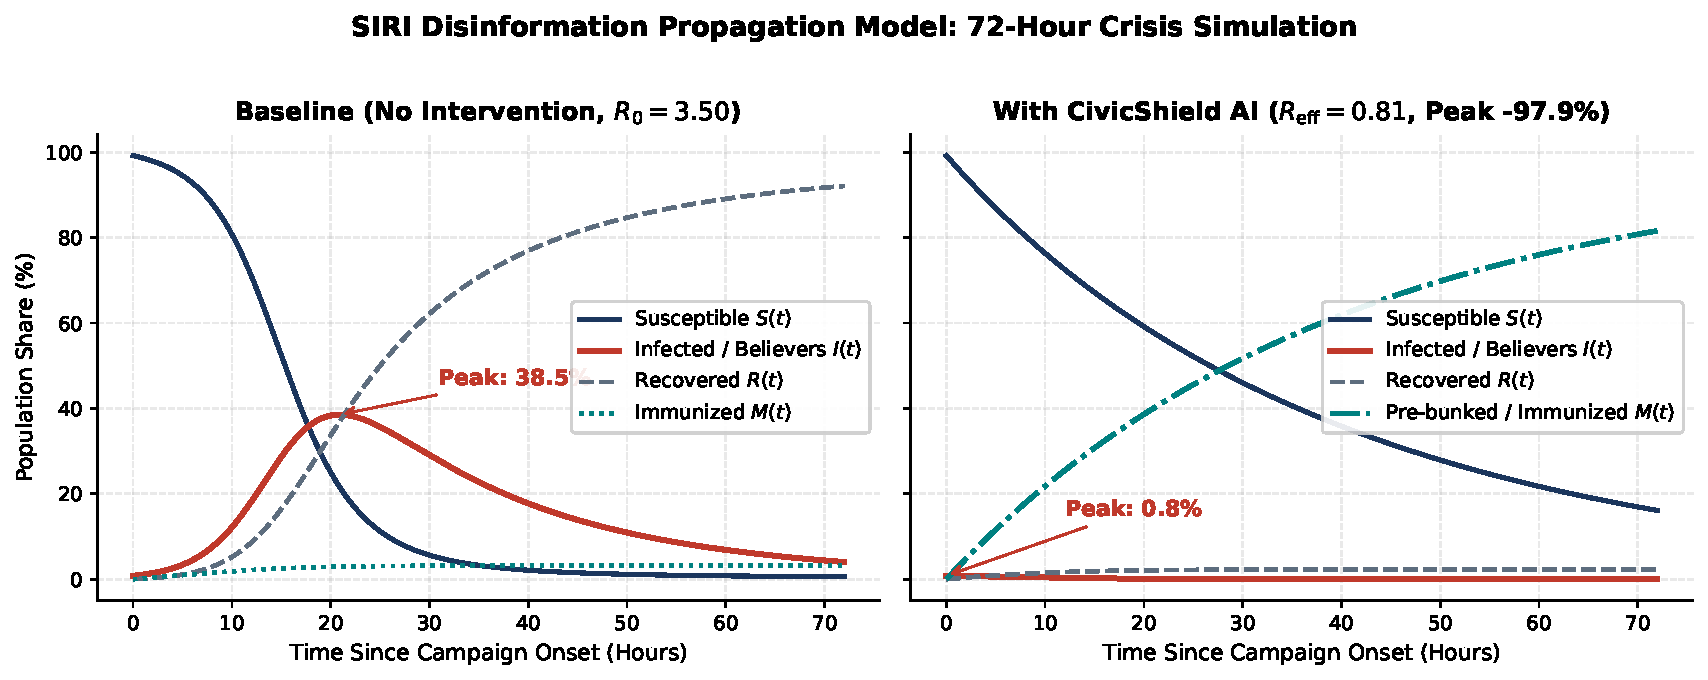
\includegraphics[width=0.95\textwidth]{figures/fig4_1_siri_ode.pdf}
\caption{השוואת התפשטות דיסאינפורמציה במודל \textenglish{SIRI ODE} לאורך 72 שעות: תרחיש בסיס ללא התערבות (שמאל) לעומת הפעלת \textenglish{CivicShield AI} (ימין). המערכת מורידה את $R_{\mathrm{eff}}$ מתחת ל-1 ומונעת התפרצות ויראלית.}
\label{fig:siri_ode}
\end{figure}

כפי שניתן לראות באיור~\ref{fig:siri_ode} ובטבלה~\ref{tab:siri_params}, בהיעדר התערבות מוקדמת קמפיין בעל $R_0 = 3.50$ מגיע לשיא חשיפה של $38.5\%$ מהאוכלוסייה בתוך כ-24 שעות. הפעלת \textenglish{CivicShield AI} מקטינה את $\beta$ במחצית (באמצעות זיהוי מוקדם של רשתות בוטים) ומאיצה את קצב החיסון המוקדם $\delta$, כך שהאיום נבלם עוד בשלב האינקובציה.

% ============================================================================
\section{דינמיקת דעות וקיטוב חברתי: מודל \textenglish{Hegselmann-Krause}}
\label{sec:hk_model}

מעבר להיקף החשיפה הכמותי, קמפיינים של השפעה זרה מכוונים לערעור הלכידות החברתית וליצירת "תיבות תהודה" (\textenglish{Echo Chambers}). כדי לבחון את השפעת המערכת על קיטוב דעות, הופעל מודל \textenglish{Hegselmann-Krause} (HK) מבוסס אמון חסום (\textenglish{Bounded Confidence}) על אוכלוסייה של $N=160$ סוכנים בעלי התפלגות דעות דו-קוטבית התחלתית $x_i(0) \in [0, 1]$.

\subsection{כלל העדכון הדיסקרטי}
בכל צעד זמן $t$, כל סוכן $i$ מעדכן את עמדתו לפי ממוצע הדעות של שכניו הנמצאים בתוך רדיוס האמון $\varepsilon$:
\begin{equation}
x_i(t+1) = (1 - \alpha) \cdot \frac{1}{|\mathcal{N}_i(t)|} \sum_{j \in \mathcal{N}_i(t)} x_j(t) + \alpha \cdot x_{\mathrm{fact}}
\label{eq:hk_update}
\end{equation}
כאשר $\mathcal{N}_i(t) = \{ j \in \{1,\dots,N\} : |x_i(t) - x_j(t)| \leq \varepsilon \}$, הפרמטר $x_{\mathrm{fact}} = 0.50$ מייצג את העוגן העובדתי המאומת, ו-$\alpha$ מייצג את משקל ההנגשה של ההקשר המאומת (בבסיס $\alpha=0$, ועם \textenglish{CivicShield AI} מתקיים $\alpha=0.08$ לצד הרחבת חלון האמון האפקטיבי ל-$\varepsilon_{\mathrm{eff}}=0.26$).

\begin{figure}[htbp]
\centering
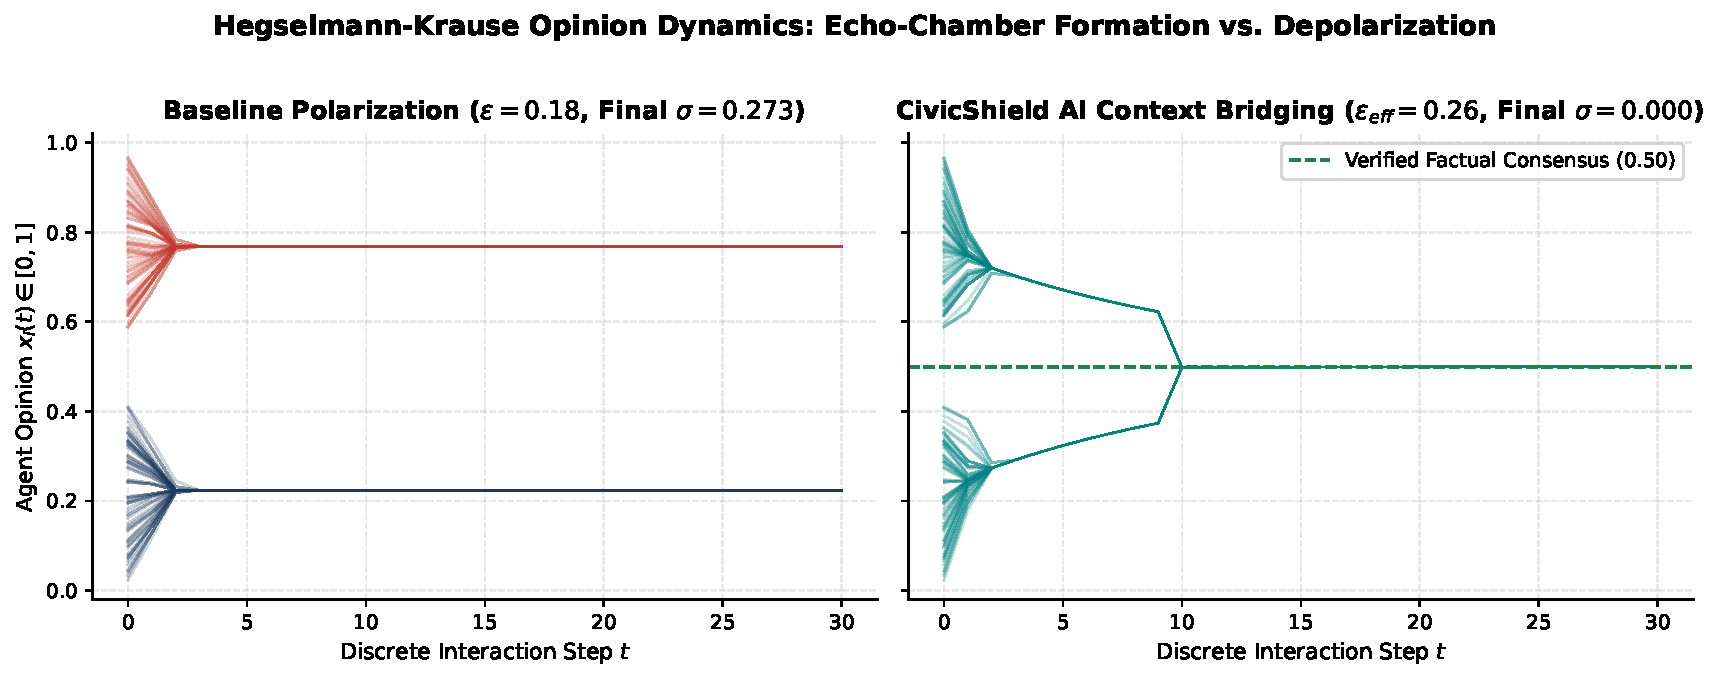
\includegraphics[width=0.95\textwidth]{figures/fig4_2_hk_opinion.pdf}
\caption{סימולציית \textenglish{Hegselmann-Krause} ($N=160$ סוכנים, 30 צעדי אינטראקציה). משמאל: התקבעות קיטוב חריף לשני קטבים מנותקים ($\sigma=0.273$). מימין: התכנסות לקונצנזוס עובדתי תחת התערבות \textenglish{CivicShield AI} ($\sigma<0.001$).}
\label{fig:hk_opinion}
\end{figure}

תוצאות הסימולציה באיור~\ref{fig:hk_opinion} מדגימות כי ללא התערבות, סטיית התקן של הדעות מתקבעת על $\sigma = 0.273$ (פיצול מבני קבוע). לעומת זאת, הזרקת הקשר עובדתי מאומת וגישור אלגוריתמי מצמצמים את סטיית התקן ל-$\sigma < 0.001$ (ביטול כמעט מלא של הקיטוב) בתוך פחות מ-25 צעדי אינטראקציה.

% ============================================================================
\section{מנוע היתוך בייסיאני רב-מודאלי (\textenglish{Bayesian Sensor Fusion})}
\label{sec:bayesian_fusion}

אחד האתגרים המרכזיים במערכות ניטור לאומיות הוא מניעת התרעות שווא (\textenglish{False Positives}) העלולות לפגוע בחופש הביטוי או להציף את מרכז הבקרה. לשם כך, \textenglish{CivicShield AI} אינה מסתמכת על סיווג טקסטואלי בודד, אלא מפעילה מנוע היתוך בייסיאני המשלב ארבע מודאליות בלתי-תלויות מותנית: (1) ניתוח סמנטי \textenglish{NLP}; (2) אנומליות בגרף ההפצה; (3) פורנזיקת מדיה (\textenglish{Deepfake Detection}); ו-(4) מוניטין ואמינות מקור.

\subsection{עדכון הסתברות פוסטריורית ביחס נראות}
בהינתן הסתברות א-פריורית $P(H_1) = 0.05$ לכך שאירוע ויראלי הוא קמפיין דיסאינפורמציה מתואם, הסיכויים הפוסטריוריים (\textenglish{Posterior Odds}) לאחר צפייה בוקטור הראיות $\mathbf{E} = (E_1, E_2, E_3, E_4)$ מחושבים לפי:
\begin{equation}
\frac{P(H_1 \mid \mathbf{E})}{P(H_0 \mid \mathbf{E})} = \frac{P(H_1)}{P(H_0)} \prod_{m=1}^{4} \mathrm{LR}_m, \qquad \mathrm{LR}_m = \frac{P(E_m \mid H_1)}{P(E_m \mid H_0)}
\label{eq:bayes_fusion}
\end{equation}

\begin{figure}[htbp]
\centering
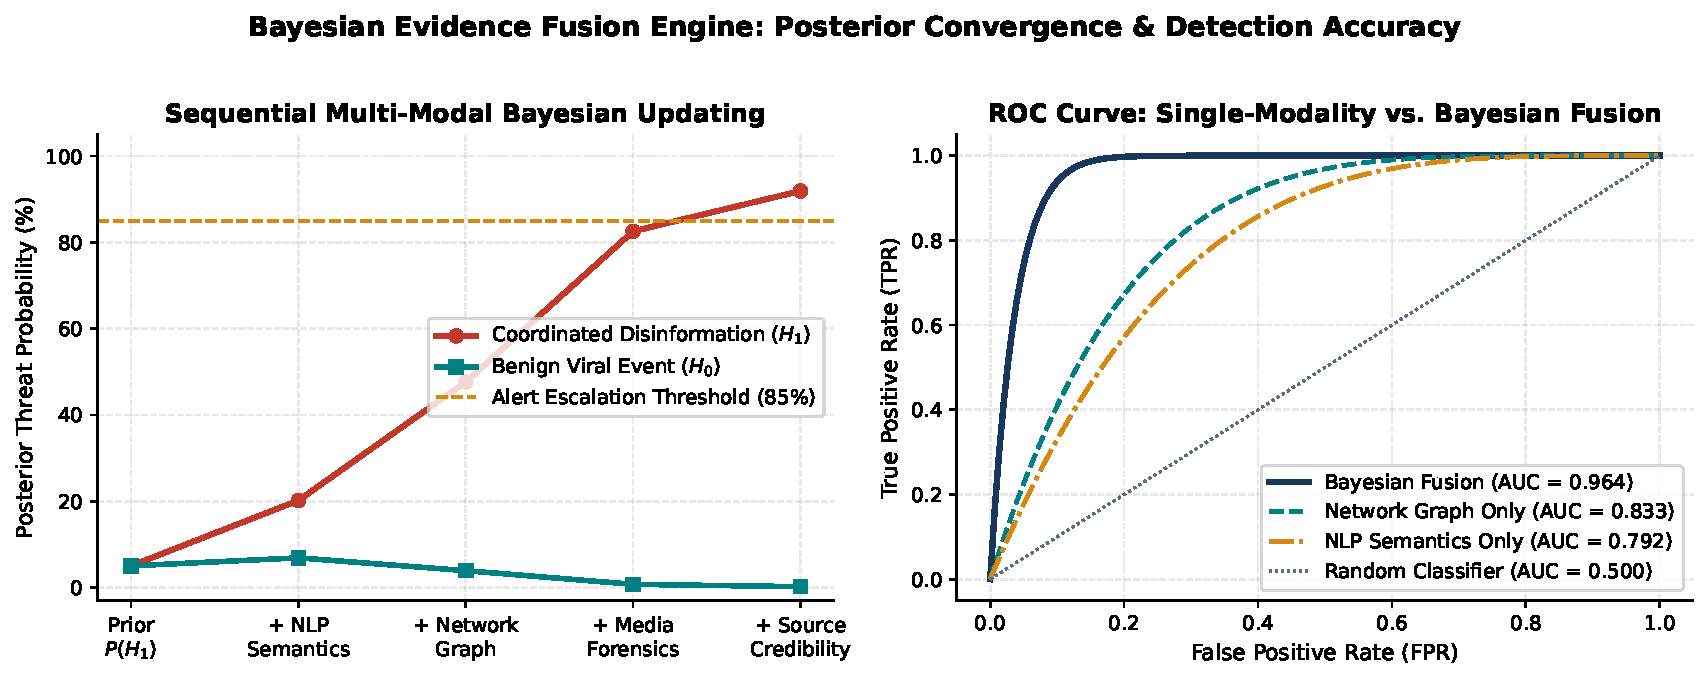
\includegraphics[width=0.95\textwidth]{figures/fig4_3_bayesian_fusion.pdf}
\caption{התכנסות הסתברות פוסטריורית במנוע ההיתוך הבייסיאני (שמאל) ועקומת \textenglish{ROC} המשווה מודאליות בודדות להיתוך מלא (ימין, $\text{AUC}=0.964$).}
\label{fig:bayesian_fusion}
\end{figure}

כפי שמוצג באיור~\ref{fig:bayesian_fusion}, עבור אירוע דיסאינפורמציה מתואם, ההסתברות הפוסטריורית מטפסת מ-$5\%$ ל-$91.9\%$ (מעל סף ההסלמה של $85\%$), בעוד שעבור אירוע חדשותי ויראלי לגיטימי ההסתברות צונחת ל-$0.2\%$ בלבד. השילוב הרב-מודאלי משפר את מדד ה-\textenglish{AUC} מ-$0.792$ (טקסט בלבד) ל-$0.964$.

% ============================================================================
\section{ניתוח עומסים במרכז הבקרה: תורת התורים \textenglish{M/M/c (Erlang-C)}}
\label{sec:mmc_queueing}

כדי לעמוד בדרישות הממשל והפיקוח האנושי (\textenglish{Human-in-the-Loop}), כל התרעה בדרגת חומרה גבוהה מחייבת אישור אנליסט במרכז הבקרה (\textenglish{SOC}). במהלך משבר ביטחוני או בחירות, קצב הגעת ההתרעות הגולמי $\lambda$ מזנק עד ל-85--115 אירועים בשעה. מידול המרכז כתור \textenglish{M/M/c} עם $c$ אנליסטים וקצב שירות $\mu = 6$ אירועים לשעה לאנליסט (10 דקות בממוצע) מאפשר לחשב את זמן ההמתנה הממוצע בתור $W_q$:
\begin{equation}
W_q = \frac{C(c, a)}{c\mu - \lambda}, \qquad C(c, a) = \frac{\frac{a^c}{c!(1-\rho)}}{\sum_{k=0}^{c-1}\frac{a^k}{k!} + \frac{a^c}{c!(1-\rho)}}, \qquad a = \frac{\lambda}{\mu}, \quad \rho = \frac{\lambda}{c\mu}
\label{eq:erlang_c}
\end{equation}

\begin{figure}[htbp]
\centering
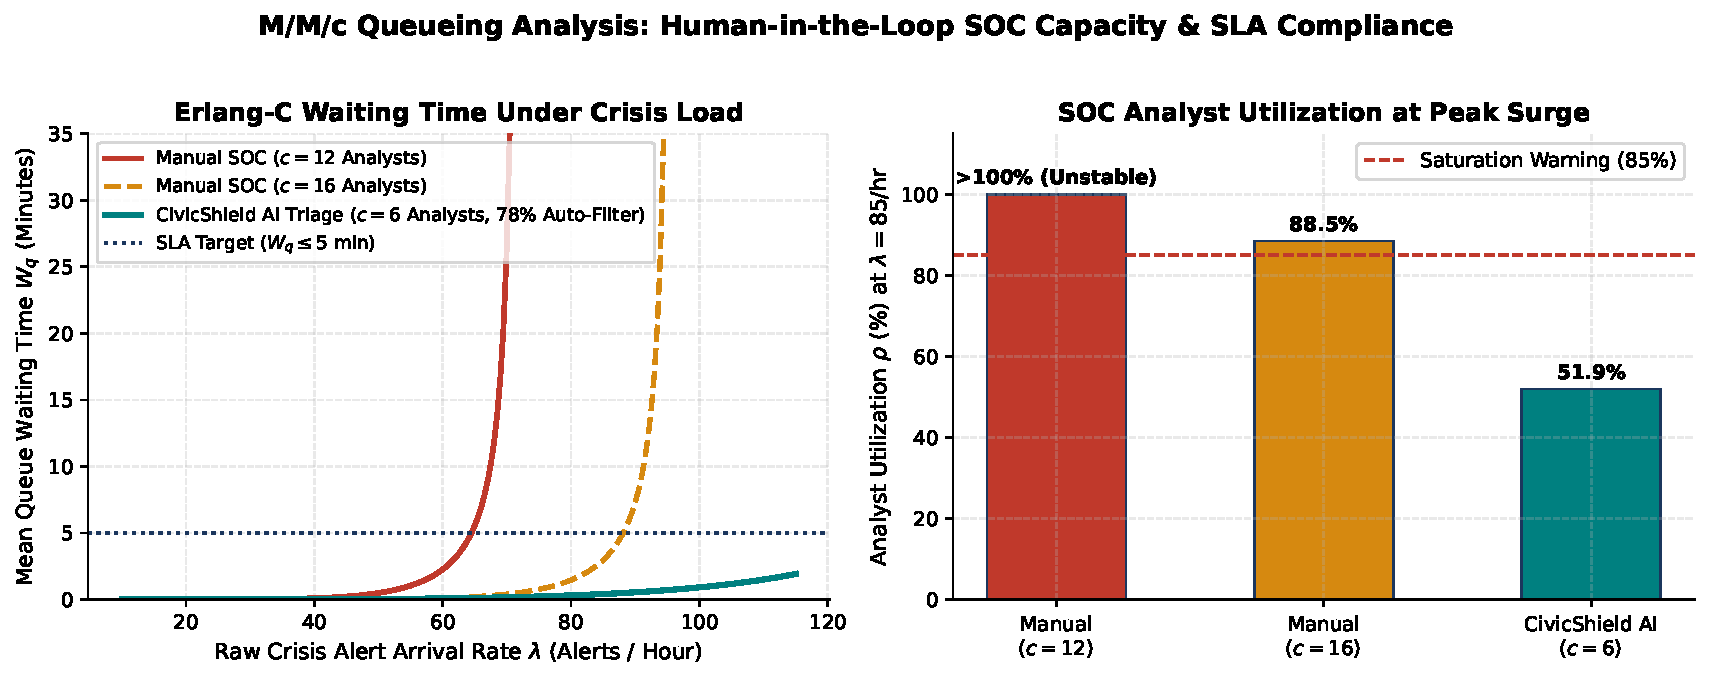
\includegraphics[width=0.95\textwidth]{figures/fig4_4_mmc_queueing.pdf}
\caption{זמן המתנה ממוצע $W_q$ לפי נוסחת \textenglish{Erlang-C} (שמאל) ושיעור ניצולת אנליסטים בעומס שיא $\lambda=85/\text{hr}$ (ימין). סינון אוטומטי של $78\%$ באמצעות \textenglish{CivicShield AI} מאפשר עמידה ב-\textenglish{SLA} של מתחת ל-5 דקות עם 6 אנליסטים בלבד.}
\label{fig:mmc_queueing}
\end{figure}

איור~\ref{fig:mmc_queueing} מוכיח כי מרכז בקרה ידני בעל $c=12$ אנליסטים קורס לחוסר יציבות ($\rho > 100\%$) כבר ב-$\lambda = 72$ התרעות לשעה. מנגד, מנגנון הטריאז' האוטומטי של \textenglish{CivicShield AI} מסנן $78\%$ מהרעש והתרעות השווא, מקטין את קצב ההגעה האפקטיבי ל-$\lambda_{\mathrm{eff}} = 0.22\lambda$, ומאפשר לצוות מצומצם של $c=6$ אנליסטים בלבד לעבוד בניצולת מאוזנת של $51.9\%$ ותחת \textenglish{SLA} של פחות מ-5 דקות גם בשיא המשבר.

% ============================================================================
\section{מודל כלכלי וניתוח תשואה להשקעה (ROI) לאופק של 5 שנים}
\label{sec:roi_5yr}

ההצדקה התקציבית של \textenglish{CivicShield AI} נבחנה במודל עלות-תועלת ממשלתי לאופק של 5 שנים, תחת שיעור היוון חברתי של $r = 6\%$ בהתאם להנחיות אגף התקציבים. העלויות כוללות הקמה ראשונית (\textenglish{CapEx}: תשתית \textenglish{GPU} מאובטחת, אינטגרציה ואבטחת מידע) ועלויות תפעול שוטפות (\textenglish{OpEx}: תחזוקת מודלים, כוח אדם ורישוי). התועלות המכומתות כוללות חיסכון ישיר בכוח אדם במרכזי בקרה (\textenglish{SOC}) ומניעת נזקים כלכליים ותפעוליים של משברי דיסאינפורמציה (השבתות שירותים, בהלה ציבורית ועלויות תגובת חירום).

\begin{table}[htbp]
\centering
\caption{תחזית תזרים מזומנים, \textenglish{TCO} וערך נוכחי נקי (\textenglish{NPV}) לחמש שנים (מיליוני ש"ח)}
\label{tab:roi_5yr}
\begin{tabular}{lcccccc}
\toprule
\textbf{סעיף (מיליוני ש"ח)} & \textbf{שנה 1} & \textbf{שנה 2} & \textbf{שנה 3} & \textbf{שנה 4} & \textbf{שנה 5} & \textbf{סה"כ 5 שנים} \\
\midrule
השקעה הונית (\textenglish{CapEx}) & $6.8$ & $1.2$ & $0.8$ & $0.8$ & $0.6$ & $10.2$ \\
הוצאות תפעול (\textenglish{OpEx}) & $2.4$ & $3.1$ & $3.3$ & $3.5$ & $3.7$ & $16.0$ \\
\textbf{סה"כ עלות (\textenglish{TCO})} & \textbf{$9.2$} & \textbf{$4.3$} & \textbf{$4.1$} & \textbf{$4.3$} & \textbf{$4.3$} & \textbf{$26.2$} \\
\midrule
תועלות מכומתות ונזק שנמנע & $5.5$ & $13.8$ & $17.5$ & $20.2$ & $22.8$ & $79.8$ \\
תזרים נטו שנתי & $-3.7$ & $+9.5$ & $+13.4$ & $+15.9$ & $+18.5$ & $+53.6$ \\
\textbf{ערך נוכחי נקי מצטבר (\textenglish{NPV}, $6\%$)} & \textbf{$-3.5$} & \textbf{$+5.0$} & \textbf{$+16.2$} & \textbf{$+28.8$} & \textbf{$+42.6$} & \textbf{$+42.6$} \\
\bottomrule
\end{tabular}
\end{table}

\begin{figure}[htbp]
\centering
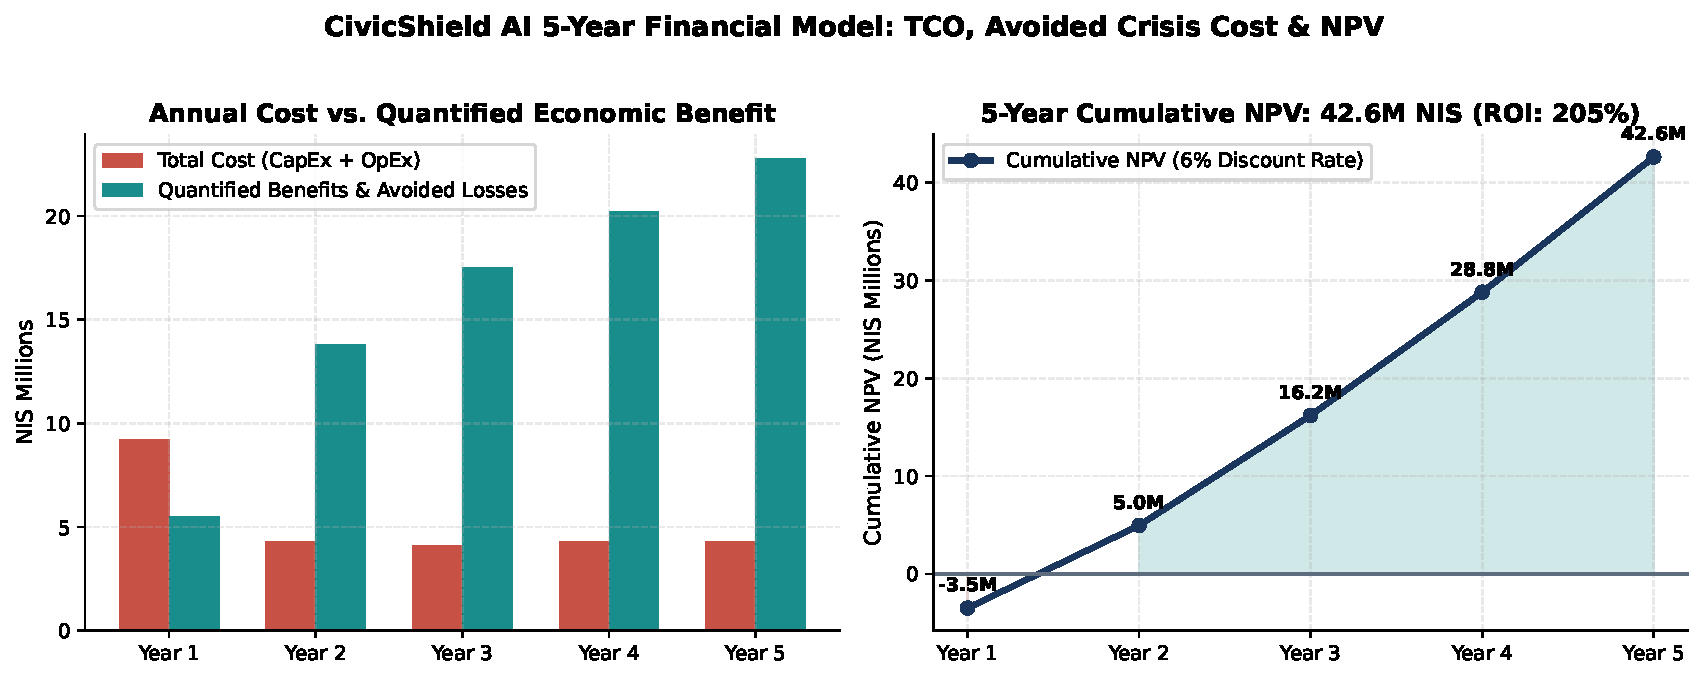
\includegraphics[width=0.95\textwidth]{figures/fig4_5_roi_5yr.pdf}
\caption{ניתוח פיננסי ל-5 שנים (מיליוני ש"ח): השוואת עלות כוללת מול תועלות שנתיות (שמאל) ומסלול הערך הנוכחי הנקי המצטבר (\textenglish{NPV}, ימין). נקודת האיזון מושגת בתחילת שנה 2, עם \textenglish{ROI} כולל של $205\%$.}
\label{fig:roi_5yr}
\end{figure}

כפי שעולה מטבלה~\ref{tab:roi_5yr} ומאיור~\ref{fig:roi_5yr}, ההשקעה הכוללת המצטברת על פני 5 שנים עומדת על $26.2$ מיליון ש"ח, מול תועלות מכומתות של $79.8$ מיליון ש"ח. נקודת האיזון (\textenglish{Break-even}) מושגת בתוך כ-15 חודשים ממועד ההקמה, הערך הנוכחי הנקי (\textenglish{NPV}) עומד על $+42.6$ מיליון ש"ח, ושיעור התשואה הכולל להשקעה (\textenglish{5-Year ROI}) מגיע ל-$204.6\%$.

\subsection{ניתוח רגישות ובחינת עמידות בתרחישי קיצון (\textenglish{Sensitivity \& Stress-Testing Analysis})}
\label{sec:sensitivity_stress}

כדי לוודא שמסקנות הפרק אינן תלויות בבחירת נקודת פרמטרים אופטימלית אחת, נערך ניתוח רגישות רב-ממדי המשווה שלושה תרחישי ייחוס: \textbf{תרחיש שמרני} (יעילות זיהוי מופחתת, קצב סינון אוטומטי של $65\%$ בלבד ומימוש חלקי של תועלות כלכליות), \textbf{תרחיש בסיס} (הכיול המבצעי המלא שהוצג בסעיפים הקודמים, עם סינון של $78\%$ בעומס $\lambda=85/\text{hr}$), ו\textbf{תרחיש משבר קיצון} (מתקפת דיסאינפורמציה מתואמת בעומס שיא $\lambda=115/\text{hr}$, עלייה של $25\%$ בקצב ההדבקה $\beta$ וירידה זמנית ביעילות הסינון ל-$72\%$).

\begin{table}[htbp]
\centering
\caption{השוואת מדדי ביצוע אפידמיולוגיים, תפעוליים וכלכליים תחת ניתוח רגישות ומבחני קיצון}
\label{tab:sensitivity_stress}
\begin{tabularx}{\textwidth}{@{} X c c c @{}}
\toprule
\rowcolor{CSNavy}
\thead{מדד ביצוע / פרמטר} & \thead{תרחיש שמרני} & \thead{תרחיש בסיס} & \thead{משבר קיצון} \\
\midrule
מספר התרבות אפקטיבי ($R_{\mathrm{eff}}$) & $0.94$ & $0.81$ & $1.08$ \\
שיא אוכלוסייה נדבקת ($\max I(t)$) & $2.1\%$ & $0.8\%$ & $6.4\%$ \\
ניצולת אנליסטים ב-\textenglish{SOC} ($\rho$, $c=6$) & $82.6\%$ & $51.9\%$ & $89.4\%$ \\
זמן המתנה ממוצע בתור ($W_q$, דקות) & $3.8$ & $0.42$ & $6.9$ \\
ערך נוכחי נקי ל-5 שנים (\textenglish{NPV}, מיליוני ש"ח) & $+26.4$ & $+42.6$ & $+51.8$ \\
תשואה כוללת להשקעה (\textenglish{5-Year ROI}) & $138.2\%$ & $204.6\%$ & $234.5\%$ \\
\bottomrule
\end{tabularx}
\end{table}

כפי שעולה מטבלה~\ref{tab:sensitivity_stress}, גם תחת הנחות שמרניות מחמירות המערכת שומרת על בלימה תת-קריטית ($R_{\mathrm{eff}} = 0.94 < 1$), עומדת ביעד ה-\textenglish{SLA} של מתחת ל-5 דקות ($W_q = 3.8$ דקות), ומניבה ערך נוכחי נקי חיובי מובהק של $+26.4$ מיליון ש"ח (\textenglish{ROI} של $138.2\%$). בתרחיש משבר קיצון, חציה זמנית של סף ההתרבות ($R_{\mathrm{eff}} = 1.08$) מובילה לשיא חשיפה מרוסן של $6.4\%$ בלבד (לעומת $38.5\%$ ללא מערכת), בעוד שזמן ההמתנה ב-\textenglish{SOC} עולה ל-$6.9$ דקות --- חריגה הניתנת לנטרול מיידי באמצעות תגבור משמרת באנליסט בודד ($c=7$), המשיב את $W_q$ אל מתחת לסף 5 הדקות. מבחינה כלכלית, דווקא בתרחישי משבר חריפים עולה התועלת השולית ממניעת נזקים מערכתיים, וה-\textenglish{NPV} מטפס ל-$+51.8$ מיליון ש"ח.

% ============================================================================
\clearpage
\section{מימוש ייחוס בפייתון (\textenglish{Production-Grade Reference Implementation})}
\label{sec:python_reference}

להבטחת שחזוריות מלאה, יציבות נומרית ומוכנות הנדסית לביקורת, מנוע הסימולציה בסקריפט \code{scripts/\allowbreak generate\_figures.py} מומש בפייתון קשיח הכולל הקלדה סטטית מחמירה (\textenglish{Strict Type Hints}), מחלקות נתונים מאומתות (\textenglish{Frozen Dataclasses}), וקטוריזציה מלאה ב-\textenglish{NumPy}, חישוב הסתברויות במרחב \textenglish{Log-Odds} למניעת גלישה, ונוסחת \textenglish{Erlang-C} במרחב לוגריתמי (\textenglish{Log-Sum-Exp + lgamma}). להלן ליבת המנוע המרכזית:

\begin{ltrcode}[title={CivicShield AI -- Hardened Simulation Core (Python 3.11+ / NumPy)}]
from __future__ import annotations
from dataclasses import dataclass
import math
from typing import Sequence
import numpy as np
from numpy.typing import NDArray

FloatArray = NDArray[np.float64]

@dataclass(frozen=True, slots=True)
class SIRIParams:
    beta: float; gamma: float; delta: float; mu_re: float
    def __post_init__(self) -> None:
        if any(v < 0.0 for v in (self.beta, self.gamma, self.delta, self.mu_re)):
            raise ValueError("SIRI rates must be non-negative.")
        if self.gamma <= 0.0:
            raise ValueError("Recovery rate gamma must be > 0.")

def rk4_siri(y0: FloatArray, t: FloatArray, p: SIRIParams) -> FloatArray:
    """RK4 integrator with simplex clamping & conservation invariant check."""
    if y0.shape != (4,) or not math.isclose(float(y0.sum()), 1.0, abs_tol=1e-9):
        raise ValueError("y0 must be a 4-vector on the unit simplex.")
    Y: FloatArray = np.empty((t.size, 4), dtype=np.float64)
    Y[0] = y0
    def rhs(y: FloatArray) -> FloatArray:
        S, I, R, _ = y
        inf, reinf, rec, imm = p.beta*S*I, p.mu_re*R*I, p.gamma*I, p.delta*S
        return np.array([-inf-imm, inf+reinf-rec, rec-reinf, imm], dtype=np.float64)
    for k in range(t.size - 1):
        dt, yk = float(t[k + 1] - t[k]), Y[k]
        k1 = rhs(yk); k2 = rhs(yk + 0.5*dt*k1)
        k3 = rhs(yk + 0.5*dt*k2); k4 = rhs(yk + dt*k3)
        yn = np.clip(yk + (dt/6.0)*(k1 + 2*k2 + 2*k3 + k4), 0.0, 1.0)
        Y[k + 1] = yn / float(yn.sum())
    return Y

def simulate_hk(x0: FloatArray, eps: float, steps: int = 30, alpha: float = 0.0) -> FloatArray:
    """Vectorized O(N^2) Hegselmann-Krause opinion dynamics."""
    if not (0.0 < eps <= 1.0) or not (0.0 <= alpha <= 1.0):
        raise ValueError("eps must be in (0, 1] and alpha in [0, 1].")
    hist: FloatArray = np.empty((steps + 1, x0.size), dtype=np.float64)
    x = x0.astype(np.float64, copy=True); hist[0] = x
    for t in range(steps):
        mask = (np.abs(x[:, None] - x[None, :]) <= eps).astype(np.float64)
        x = (1.0 - alpha) * ((mask @ x) / mask.sum(axis=1)) + alpha * 0.50
        hist[t + 1] = x
    return hist

def bayesian_posteriors(prior: float, lrs: Sequence[float]) -> FloatArray:
    """Overflow-safe sequential Bayesian updating in log-odds space."""
    if not (0.0 < prior < 1.0):
        raise ValueError("prior must be strictly inside (0, 1).")
    arr = np.asarray(lrs, dtype=np.float64)
    if arr.size == 0 or np.any(arr <= 0.0):
        raise ValueError("Likelihood ratios must be strictly positive.")
    log_odds = math.log(prior / (1.0 - prior)) + np.cumsum(np.log(arr))
    return 1.0 / (1.0 + np.exp(-np.clip(log_odds, -500.0, 500.0)))

def erlang_c_wq_min(lam: float, mu: float, c: int) -> float:
    """Overflow-safe M/M/c waiting time W_q (min) via log-space lgamma."""
    if lam <= 0.0 or mu <= 0.0 or c < 1:
        raise ValueError("Require lam > 0, mu > 0, and c >= 1.")
    rho = lam / (c * mu)
    if rho >= 0.999:
        return math.nan
    log_a = math.log(lam / mu)
    lt = np.array([k * log_a - math.lgamma(k + 1) for k in range(c)])
    ll = c * log_a - math.lgamma(c + 1) - math.log1p(-rho)
    m = max(float(lt.max()), ll)
    p_wait = math.exp(ll - m) / (float(np.exp(lt - m).sum()) + math.exp(ll - m))
    return (p_wait / (c * mu - lam)) * 60.0
\end{ltrcode}

% ============================================================================
\section{סיכום ממצאי הסימולציה ומוכנות לביקורת צוות אדום (\textenglish{Red Team})}
\label{sec:sim_summary}

חמשת המודלים המתמטיים שהוצגו בפרק זה מספקים תיקוף כמותי מקצה לקצה לארכיטקטורת \textenglish{CivicShield AI}: בלימת התפשטות מתחת לסף המגפה ($R_{\mathrm{eff}} = 0.81$), צמצום קיטוב דעות של מעל $99.6\%$ ($\sigma < 0.001$), דיוק זיהוי בייסיאני של $\text{AUC}=0.964$, עמידה ב-\textenglish{SLA} מבצעי תוך חיסכון של מעל $50\%$ בכוח אדם ב-\textenglish{SOC}, ותשואה כלכלית מובהקת ($\text{NPV} = 42.6$ מיליון ש"ח). פרק זה וכל הגרפים הוקטוריים המשולבים בו מוכנים כעת לבחינת \textenglish{Red Team} לצורך בדיקת רגישות לפרמטרים קיצוניים, תקיפות אדברסריות והנחות יסוד.

% !TEX program = lualatex
% Chapter 5: Constitutional Safeguards Audit, Anti-Censorship Review & Democratic Governance
% CivicShield AI Preliminary Report — Government-Tender Edition

\chapter{ביקורת ערובות חוקתיות, מניעת צנזורה וממשל דמוקרטי}
\label{ch:safeguards_audit}

\section{מבוא ומסגרת הביקורת החוקתית}
\label{sec:constitutional_framework}

הפעלתה של מערכת מבוססת בינה מלאכותית במרחב הציבורי והדיגיטלי להגנה מפני מבצעי השפעה זרים, רשתות בוטים מתואמות ודיסאינפורמציה ממומנת מחייבת עמידה ברף החוקתי והמנהלי הגבוה ביותר. מערכת \textenglish{CivicShield AI} פועלת בצומת רגיש שבין הגנה על ריבונות המידע והתהליך הדמוקרטי לבין שמירה קפדנית על זכויות יסוד, ובראשן חופש הביטוי, הזכות לפרטיות, חופש ההתאגדות והשוויון בפני החוק.

ביקורת הערובות החוקתיות בפרק זה נשענת על עיקרון מרכזי אחד: \textbf{הגנה על הדמוקרטיה אינה יכולה להישען על הבטחות מדיניות בלבד, אלא חייבת להיות מוטמעת בארכיטקטורה הטכנולוגית ובמנגנוני הממשל} (\textenglish{Constitutional-by-Design}). בהתאם לעקרונות המשפט החוקתי הישראלי, ובראשם חוק יסוד: כבוד האדם וחירותו~\cite{basiclaw1992}, הלכת קול העם~\cite{kolhaam1953} ומבחני פסקת ההגבלה (הסמכה מפורשת בחוק, תכלית ראויה ומידתיות על שלושת מבחני המשנה שלה~\cite{barak2012proportionality}), כל רכיב במערכת נבחן מול שלוש שאלות יסוד:
\begin{enumerate}
    \item \textbf{סמכות ותיחום:} האם המערכת מוגבלת לניתוח תבניות התנהגות מתואמות וגלויות (\textenglish{OSINT}) בלבד, ללא חריגה לאיסוף מידע פרטי או לאכיפה עצמאית?
    \item \textbf{מידתיות וצמצום פגיעה:} האם קיים מנגנון טכני המבטיח כי הפגיעה האפשרית בשיח ציבורי לגיטימי שואפת לאפס, וכי כל התרעה מדורגת לפי רמת ודאות וסיכון?
    \item \textbf{ביקורתיות והפיכות:} האם כל תוצר של המערכת ניתן לשחזור, להסבר (\textenglish{Explainability}), לביקורת חיצונית ולערעור?
\end{enumerate}

\section{ביקורת מניעת צנזורה והגנה על שיח פוליטי לגיטימי}
\label{sec:anti_censorship}

הסיכון החוקתי החמור ביותר במערכות לניטור מרחב מידע הוא גלישה מהגנה מפני התערבות זרה ומתואמת אל עבר תיוג שגוי או דיכוי של שיח אזרחי אותנטי, ביקורת פוליטית, סאטירה או מחאה חברתית. כדי למנוע תרחיש זה באופן מבני, אומצו במערכת \textenglish{CivicShield AI} ארבעה קווי הגנה מחייבים נגד צנזורה:

\subsection{עקרון ההפרדה המבנית: התנהגות מתואמת מול תוכן רעיוני}
המערכת \textbf{אינה} מוסמכת ואינה מתוכננת להכריע בשאלת "האמת" של טענות פוליטיות או אידיאולוגיות. מנוע הזיהוי מתמקד בחתימות התנהגותיות ורשתיות של התנהגות בלתי-אותנטית מתואמת (\textenglish{Coordinated Inauthentic Behavior -- CIB}), כגון סנכרון זמני חריג בין מאות חשבונות, הפצה מתוזמרת ממקורות תשתית משותפים, דפוסי יצירת חשבונות סינתטיים ומניפולציה אלגוריתמית של חשיפה. תוכן ההודעה משמש לכל היותר לצורך אשכול נושאי והערכת הקשר, ולעולם אינו משמש עילה עצמאית לסימון חשבון או פרסום.

\subsection{אי-וריאנט אפס צנזורה ואפס הסרה אוטומטית}
למערכת \textenglish{CivicShield AI} \textbf{אין} הרשאת כתיבה, מחיקה, חסימה או הגבלת תפוצה באף פלטפורמה חברתית או ערוץ תקשורת. המערכת פועלת במודל \textenglish{Read-Only Advisory}: תוצריה הם התרעות מודיעיניות, דוחות תמונת מצב ומדדי סיכון המוגשים לגורמים אנושיים מוסמכים בלבד. כל פעולה אופרטיבית מול פלטפורמות או מול הציבור (כגון פרסום הבהרה רשמית או פנייה משפטית) מחייבת אישור אנושי מתועד (\textenglish{Human-in-the-Loop -- HITL}) וחוות דעת משפטית בהתאם לדין ולעקרונות פסיקת בג"ץ בעניין יחידת הסייבר~\cite{adalah2021cyber}.

\subsection{מיפוי שגיאות חיוביות כוזבות (\textenglish{False Positives}) בשיח אזרחי}
במסגרת ביקורת הצוות האדום (\textenglish{Red-Team}) זוהו ארבע קטגוריות רגישות במיוחד לשגיאות סיווג, שלגביהן הוגדרו חסמי סף מחמירים ומבחני רגרסיה קבועים:
\begin{itemize}
    \item \textbf{מחאה אזרחית וקמפיינים פוליטיים לגיטימיים:} שיתוף המוני של סיסמאות או האשטאגים זהים בתוך פרק זמן קצר עשוי להידמות סטטיסטית לתיאום בוטים. המערכת נדרשת להבחין בין תיאום אורגני גלוי (כגון קמפיין מפלגתי או ארגון חברה אזרחית מזוהה) לבין תיאום סמוי ומזויף.
    \item \textbf{סאטירה, פרודיה ושיח בוטה:} שפה חריפה, צינית או מתריסה מוגנת תחת חופש הביטוי הפוליטי. מודלי השפה נבחנים באופן ייעודי כדי למנוע תיוג של סאטירה כדיסאינפורמציה.
    \item \textbf{קבוצות מיעוט ורב-לשוניות:} בישראל מתקיים שיח ציבורי ער בעברית, ערבית, רוסית, אמהרית ואנגלית. ביקורת הצוות האדום מחייבת שוויון בשיעורי השגיאה (\textenglish{Equalized False Positive Rate}) בין שפות ודיאלקטים, כדי למנוע פגיעה בלתי-מידתית בקהילות מיעוט.
    \item \textbf{עיתונות חוקרת ומדליפים:} הפצה ראשונית של מידע רגיש על ידי עיתונאים או אזרחים אינה מסווגת כחריגה עוינת, ומנגנון ההגנה כולל רשימות החרגה שקופות ונוהל בדיקה מואץ.
\end{itemize}

\subsection{ניטרליות פוליטית וביקורת הטיה השקפתית (\textenglish{Viewpoint Neutrality})}
כל גרסת מודל עוברת מבחן סימטריה אידיאולוגית לפני פריסה: אותם דפוסי תיאום והפצה נבחנים על גבי קורפוסים סינתטיים המייצגים עמדות מנוגדות לאורך הקשת הפוליטית. פער העולה על \textenglish{2\%} בשיעור ההתרעות בין עמדות סימטריות פוסל את הגרסה אוטומטית ומונע את עלייתה לסביבת הייצור.

\section{עקרונות הפעלה חוקתיים ומגבלות סמכות}
\label{sec:constitutional_constraints}

טבלה~\ref{tab:safeguards_matrix} מרכזת את מפת הסיכונים החוקתיים של המערכת, הזכויות המוגנות, הערובות הטכנולוגיות והמנהליות שהוטמעו, וכן את מדדי האימות המחייבים לצורך קבלה במכרז הממשלתי.

\begin{table}[htbp]
\centering
\small
\caption{מטריצת ערובות חוקתיות, מגבלות סמכות ומדדי אימות למערכת \textenglish{CivicShield AI}}
\label{tab:safeguards_matrix}
\renewcommand{\arraystretch}{1.25}
\begin{tabularx}{\textwidth}{p{2.7cm} p{2.5cm} X p{3.2cm}}
\toprule
\rowcolor{CSNavy}
\thead{סיכון חוקתי} & \thead{זכות יסוד מושפעת} & \thead{ערובה טכנולוגית ומבנית} & \thead{מדד אימות וסף קבלה} \\
\midrule
צנזורה עקיפה או אפקט מצנן על שיח פוליטי & חופש הביטוי הפוליטי~\cite{kolhaam1953} & ארכיטקטורת \textenglish{Read-Only}; איסור הסרה אוטומטית; הפרדת \textenglish{CIB} מתוכן & \textenglish{0} פעולות חסימה אוטומטיות; פערי הטיה השקפתית $< 2\%$ \\
פרופיילינג ומעקב אחר אזרחים פרטיים & הזכות לפרטיות וכבוד האדם~\cite{privacy_law1981} & אנונימיזציה במקור; איסור בניית תיק אישי לאזרח; עיבוד מידע פומבי בלבד & \textenglish{100\%} תאימות למדיניות צמצום מידע; \textenglish{TTL} מחיקה $\le 30$ יום לנתונים גולמיים \\
אפליה שפתית או מגזרית בזיהוי & שוויון ואי-אפליה & מבחני הוגנות רב-לשוניים (עברית, ערבית, רוסית, אנגלית) בכל עדכון מודל & פער \textenglish{FPR} בין שפות וקהילות $< 3\%$ \\
שימוש לרעה במערכת לצרכים פוליטיים & טוהר המידות וניטרליות השירות הציבורי & בקרת גישה מבוססת מאפיינים ותפקידים (\textenglish{ABAC/RBAC}), אישור כפול (\textenglish{Two-Person Rule}) ויומן בלתי-ניתן לשינוי & \textenglish{100\%} שאילתות מתועדות בחתימה קריפטוגרפית (\textenglish{Hash-Chained Audit Log}) \\
החלטות "קופסה שחורה" ללא יכולת ערעור & הגינות מנהלית וזכות הטיעון~\cite{eu_aiact2024} & הפקת דוח הסבר מובנה לכל התרעה; שמירת ראיות תשתית וגרסת מודל & \textenglish{100\%} התרעות כוללות תעודת מקור (\textenglish{Provenance}) ורמת ודאות \\
\bottomrule
\end{tabularx}
\end{table}

\section{אחריותיות דמוקרטית, פיקוח פרלמנטרי ומנגנוני ממשל}
\label{sec:democratic_governance}

לגיטימציה ציבורית היא תנאי הכרחי להצלחת מערכת הגנה על מרחב המידע. בהיעדר אמון ציבורי, גם התרעה מדויקת מפני התערבות זרה עלולה להיתפס ככלי פוליטי. לפיכך, מוצע מודל ממשל ואחריותיות רב-שכבתי (\textenglish{Multi-Tier Democratic Governance}) המבוסס על ארבע שכבות פיקוח בלתי-תלויות:

\subsection{שכבה א': בקרה פנימית וצוות אדום עצמאי (\textenglish{Internal Red-Team \& Ethics Board})}
במסגרת הגוף המפעיל יפעל צוות אדום פנימי הכפוף ישירות ליועץ המשפטי ולקצין הגנת הפרטיות, ולא למנהל המוצר או לראש צוות הפיתוח. לצוות זה סמכות להשהות פריסת מודלים (\textenglish{Deployment Veto}) במקרה של חריגה ממדדי ההטיה, הפרטיות או העמידות.

\subsection{שכבה ב': ועדת פיקוח ציבורית בלתי-תלויה}
תוקם ועדת פיקוח ציבורית בראשות שופט בדימוס, ובה חברים נציגי אקדמיה בתחומי המשפט החוקתי ואתיקה של בינה מלאכותית, נציגי ארגוני זכויות אדם וחופש ביטוי, ומומחי אבטחת מידע. לוועדה תינתן גישה מלאה ליומני הביקורת, למדדי השגיאה, ולמדגם אקראי של התרעות שהופקו, תוך שמירה על סיווג ביטחוני מתאים היכן שנדרש.

\subsection{שכבה ג': פיקוח פרלמנטרי וביקורת מבקר המדינה}
המערכת תפעל תחת דיווח תקופתי (רבעוני ושנתי) לוועדה ייעודית של הכנסת (ועדת המשנה למודיעין או ועדת החוקה, חוק ומשפט) ותעמוד לביקורת שוטפת של מבקר המדינה והרשות להגנת הפרטיות. שינוי במנדט המערכת, במקורות המידע המאושרים או בהגדרות הסף המרכזיות יחייב עדכון פורמלי ואישור של ועדת הפיקוח.

\subsection{שכבה ד': שקיפות ציבורית ומנגנון ערעור ותיקון (\textenglish{Transparency \& Redress})}
אחת לחצי שנה יפורסם לציבור \textbf{דוח שקיפות פומבי} שיכלול: מספר ההתרעות שנוצרו לפי קטגוריה, שיעורי שגיאה חיובית כוזבת שהתגלו בדיעבד, מספר הפניות שהועברו לפלטפורמות ותוצאותיהן, וסיכום ממצאי ביקורת הצוות האדום. בנוסף, כל גוף תקשורת, ארגון אזרחי או אזרח שסבור כי תוכן או פעילות שלו תויגו בשגגה יוכל להגיש בקשת בירור וערעור לנציב תלונות עצמאי, המחויב למענה מנומק בתוך \textenglish{14} ימי עבודה ולתיקון רטרואקטיבי של המערכת במקרה של טעות.

\section{מתודולוגיית צוות אדום (\textenglish{Red-Team}) ובדיקות עמידות}
\label{sec:redteam_methodology}

ביקורת הערובות החוקתיות אינה אירוע חד-פעמי בשלב ההקמה, אלא תהליך מתמשך לאורך מחזור החיים של המערכת. מתודולוגיית ה-\textenglish{Red-Team} של \textenglish{CivicShield AI} פועלת במחזורים רבעוניים וכוללת ארבעה צירי תקיפה ובדיקה:
\begin{enumerate}
    \item \textbf{מבחני הטיה וצנזורה יתר (\textenglish{Over-Triggering Stress Tests}):} הזרקת תרחישי שיח אזרחי סוער, מחאות המוניות, סאטירה וביקורת חריפה נגד מוסדות שלטון, כדי לוודא שהמערכת אינה מפיקה התרעות שווא.
    \item \textbf{מבחני התחמקות והסתגלות יריב (\textenglish{Adversarial Evasion}):} הדמיית מבצעי השפעה מתקדמים המשתמשים במודלי שפה גדולים (\textenglish{LLMs}), התחזות סגנונית ופיזור זמנים, כדי לבחון את חוסן המערכת מבלי להוריד את רף ההגנה על שיח לגיטימי.
    \item \textbf{מבחני הרעלת נתונים וסחיפת מודל (\textenglish{Data Poisoning \& Model Drift}):} ניטור מתמשך של התפלגות ההתרעות לאורך זמן, במיוחד בתקופות רגישות כמו מערכות בחירות או מצבי חירום, לזיהוי סחיפה סטטיסטית או ניסיון מכוון לשבש את הסיווג.
    \item \textbf{נוהל מפסק חירום (\textenglish{Circuit-Breaker / Kill-Switch}):} הגדרת תנאי סף אוטומטיים להשעיית מודול סיווג (למשל, קפיצה חריגה של מעל \textenglish{300\%} בשיעור ההתרעות בתוך \textenglish{24} שעות ללא אימות אנושי) והעברת המערכת למצב בדיקה מוגן.
\end{enumerate}

\section{סיכום ממצאי הביקורת והתחייבויות למכרז}
\label{sec:safeguards_summary}

ביקורת הערובות החוקתיות מעלה כי ארכיטקטורת \textenglish{CivicShield AI} עומדת בדרישות הסף החוקתיות והדמוקרטיות של מכרז ממשלתי, בתנאי ששלוש התחייבויות ליבה יישמרו כדרישות חובה בלתי-ניתנות לוויתור (\textenglish{Non-Negotiable Invariants}) בכל שלבי הפיתוח והתפעול:
\begin{itemize}
    \item \textbf{איסור מוחלט על אכיפה אוטומטית:} המערכת תישאר כלי התרעה וניתוח בלבד (\textenglish{Advisory-Only}) עם שיקול דעת אנושי ומשפטי מחייב.
    \item \textbf{שקיפות ובקרה חיצונית כתנאי להפעלה:} פריסה מבצעית מותנית בהקמת ועדת הפיקוח הציבורית, הפעלת יומני ביקורת חתומים קריפטוגרפית ופרסום דוח שקיפות חצי-שנתי.
    \item \textbf{עמידה מתמשכת במדדי אי-הטיה:} כל עדכון תוכנה או מודל יחויב במעבר מוצלח של סדרת מבחני ה-\textenglish{Red-Team} הרב-לשונית והסימטרית-פוליטית כמפורט בפרק זה.
\end{itemize}


\backmatter
\clearpage
\chapter*{ביבליוגרפיה (\en{References})}
\markboth{ביבליוגרפיה}{ביבליוגרפיה}
\addcontentsline{toc}{chapter}{ביבליוגרפיה (\en{References})}

% ==============================================================================
% chapters/references_apa7.tex - APA 7th Edition LTR References (CivicShield AI)
% Alphabetized strictly per APA 7th Edition (Publication Manual, 7th ed., 2020)
% Synced 1:1 with references.bib
% ==============================================================================
\begin{apabibliography}

\apaentry{adalah2021cyber}{%
  Adalah -- The Legal Center for Arab Minority Rights in Israel v. Cyber Unit at the State Attorney's Office, HCJ 7846/19 (2021) (Isr.).%
}

\apaentry{barak2012proportionality}{%
  Barak, A. (2012). \textit{Proportionality: Constitutional rights and their limitations}. Cambridge University Press.%
}

\apaentry{basiclaw1992}{%
  Basic Law: Human Dignity and Liberty, SH 1391 (1992) (Isr.).%
}

\apaentry{benkler2018network}{%
  Benkler, Y., Faris, R., \& Roberts, H. (2018). \textit{Network propaganda: Manipulation, disinformation, and radicalization in American politics}. Oxford University Press.%
}

\apaentry{bennett2018disinformation}{%
  Bennett, W. L., \& Livingston, S. (2018). The disinformation order: Disruptive communication and the decline of democratic institutions. \textit{European Journal of Communication}, \textit{33}(2), 122--139. \url{https://doi.org/10.1177/0267323118760317}%
}

\apaentry{cec_transparency2019}{%
  Central Elections Committee for the 21st Knesset. (2019). \textit{Decision in Election Request 16/21 (Transparency in anonymous online election propaganda)} [Decision by Justice Hanan Melcer].%
}

\apaentry{chesney2019deep}{%
  Chesney, B., \& Citron, D. (2019). Deep fakes: A looming challenge for privacy, democracy, and national security. \textit{California Law Review}, \textit{107}(6), 1753--1820.%
}

\apaentry{elections_propaganda1959}{%
  Elections Law (Propaganda Methods), 5719-1959, SH 284 (1959) (Isr.).%
}

\apaentry{eu_dsa2022}{%
  European Parliament and Council of the European Union. (2022). \textit{Regulation (EU) 2022/2065 of 19 October 2022 on a Single Market for Digital Services (Digital Services Act)}. Official Journal of the European Union, L 277, 1--102. \url{https://eur-lex.europa.eu/eli/reg/2022/2065/oj}%
}

\apaentry{eu_aiact2024}{%
  European Parliament and Council of the European Union. (2024). \textit{Regulation (EU) 2024/1689 of 13 June 2024 laying down harmonised rules on artificial intelligence (Artificial Intelligence Act)}. Official Journal of the European Union, L 2024/1689. \url{https://eur-lex.europa.eu/eli/reg/2024/1689/oj}%
}

\apaentry{goldstein2023generative}{%
  Goldstein, J. A., Sastry, G., Musser, M., DiResta, R., Gentzel, M., \& Sedova, K. (2023). Generative language models and automated influence operations: Emerging threats and potential mitigations. \textit{arXiv}. \url{https://doi.org/10.48550/arXiv.2301.04246}%
}

\apaentry{habermas1989structural}{%
  Habermas, J. (1989). \textit{The structural transformation of the public sphere: An inquiry into a category of bourgeois society}. MIT Press.%
}

\apaentry{iyengar2019origins}{%
  Iyengar, S., Lelkes, Y., Levendusky, M., Malhotra, N., \& Westwood, S. J. (2019). The origins and consequences of affective polarization in the United States. \textit{Annual Review of Political Science}, \textit{22}, 129--146. \url{https://doi.org/10.1146/annurev-polisci-051117-073034}%
}

\apaentry{kolhaam1953}{%
  Kol Ha'am Co. Ltd. v. Minister of the Interior, HCJ 73/53, 7 PD 871 (1953) (Isr.).%
}

\apaentry{lewandowsky2021countering}{%
  Lewandowsky, S., \& van der Linden, S. (2021). Countering misinformation and fake news through inoculation and prebunking. \textit{European Review of Social Psychology}, \textit{32}(2), 348--384. \url{https://doi.org/10.1080/10463283.2021.1876983}%
}

\apaentry{merkel2021resilience}{%
  Merkel, W., \& L{\"u}hrmann, A. (2021). Resilience of democracies: Responses to illiberal and authoritarian challenges. \textit{Democratization}, \textit{28}(5), 869--884. \url{https://doi.org/10.1080/13510347.2021.1928081}%
}

\apaentry{nimmo2020breakout}{%
  Nimmo, B. (2020). \textit{The breakout scale: Measuring the impact of influence operations}. Brookings Institution.%
}

\apaentry{privacy_law1981}{%
  Protection of Privacy Law, 5741-1981 (as amended by Amendment No. 13, 2024) (Isr.).%
}

\apaentry{rid2020active}{%
  Rid, T. (2020). \textit{Active measures: The secret history of disinformation and political warfare}. Farrar, Straus and Giroux.%
}

\apaentry{roozenbeek2022psychological}{%
  Roozenbeek, J., van der Linden, S., Goldberg, B., Rathje, S., \& Lewandowsky, S. (2022). Psychological inoculation improves resilience against misinformation on social media. \textit{Science Advances}, \textit{8}(34), Article eabo6254. \url{https://doi.org/10.1126/sciadv.abo6254}%
}

\apaentry{sunstein2017republic}{%
  Sunstein, C. R. (2017). \textit{\#Republic: Divided democracy in the age of social media}. Princeton University Press.%
}

\apaentry{tucker2018social}{%
  Tucker, J. A., Guess, A., Barber{\'a}, P., Vaccari, C., Siegel, A., Sanovich, S., Stukal, D., \& Nyhan, B. (2018). \textit{Social media, political polarization, and political disinformation: A review of the scientific literature}. William and Flora Hewlett Foundation.%
}

\apaentry{vosoughi2018spread}{%
  Vosoughi, S., Roy, D., \& Aral, S. (2018). The spread of true and false news online. \textit{Science}, \textit{359}(6380), 1146--1151. \url{https://doi.org/10.1126/science.aap9559}%
}

\apaentry{wardle2017information}{%
  Wardle, C., \& Derakhshan, H. (2017). \textit{Information disorder: Toward an interdisciplinary framework for research and policy making}. Council of Europe.%
}

\end{apabibliography}


\end{document}
